 \documentclass[11pt]{article}
%\documentstyle[11pt]{article}
\usepackage{layout}
\usepackage{amssymb}
\usepackage{epsfig}
\usepackage{graphicx}
\usepackage{color}
%\usepackage{showkeys}
\usepackage{latexsym}

\setlength{\textwidth}{16.0cm} 
\setlength{\textheight}{21.0cm} 
\setlength{\evensidemargin}{ 0.5cm}
\setlength{\oddsidemargin} { 0.5cm} 
\setlength{\topmargin}{-0.5cm} \setlength{\baselineskip}  { 0.7cm}


\usepackage{amssymb}
\usepackage{algorithmicx}
\usepackage[ruled]{algorithm}
\usepackage{algpseudocode}
\usepackage{algpascal}
\usepackage{algc}

\alglanguage{pseudocode}
%%%%%%%%%%%%%%%%%%%%%%%%%%%%%%%%%%%%%%%%%%%%%%%%%%%%%%%%%%%%%%%%%%%%%%%%%%%%%%%%
%%%%%%%%%%%%%%%%%%%%

%\usepackage[counterclockwise]{rotating}
\usepackage{collectbox}

\makeatletter
\newcommand{\sqbox}{%
    \collectbox{%
        \@tempdima=\dimexpr\width-\totalheight\relax
        \ifdim\@tempdima<\z@
            \fbox{\hbox{\hspace{-.5\@tempdima}\BOXCONTENT\hspace{-.5\@tempdima}}}%
        \else
            \ht\collectedbox=\dimexpr\ht\collectedbox+.5\@tempdima\relax
            \dp\collectedbox=\dimexpr\dp\collectedbox+.5\@tempdima\relax
            \fbox{\BOXCONTENT}%
        \fi
    }%
}
\makeatother



\newenvironment{proof}[1][Proof]{\textbf{#1.} }{\ \rule{0.5em}{0.5em}}
\newcommand{\R}{I\!\!R}
\def\C{{\rm I\!C}}
\def\N{{\rm I\!N}}
\newtheorem{theorem}{Theorem}[section]
\newtheorem{acknowledgement}[theorem]{Acknowledgement}
%\newtheorem{algorithm}[theorem]{Algorithm}
\newtheorem{axiom}[theorem]{Axiom}
\newtheorem{case}[theorem]{Case}
\newtheorem{claim}[theorem]{Claim}
\newtheorem{conclusion}[theorem]{Conclusion}
\newtheorem{condition}[theorem]{Condition}
\newtheorem{conjecture}[theorem]{Conjecture}
\newtheorem{corollary}[theorem]{Corollary}
\newtheorem{criterion}[theorem]{Criterion}
\newtheorem{definition}[theorem]{Definition}
\newtheorem{example}[theorem]{Example}
\newtheorem{exercise}[theorem]{Exercise}
\newtheorem{lemma}[theorem]{Lemma}
\newtheorem{notation}[theorem]{Notation}
\newtheorem{problem}[theorem]{Problem}
\newtheorem{proposition}[theorem]{Proposition}
\newtheorem{remark}[theorem]{Remark}
\newtheorem{solution}[theorem]{Solution}
\newtheorem{summary}[theorem]{Summary}
\newcommand{\Frac}[2] {\frac{\textstyle #1} {\textstyle #2}}
\newcommand{\taumin}{\tau_{min}}
\newcommand{\taumax}{\tau_{max}}
\newcommand{\sigmin}{\sigma_{min}}
\newcommand{\sigmax}{\sigma_{max}}
 \newcommand{\halmos}{\hfill $\;\;\;\Box$\\}

\begin{document}

\title{Fast and Stable Schemes for Phase Fields Models}
\author{M. Brachet\thanks{Institut Elie Cartan de Lorraine, Universit\'e de Lorraine, Site de Metz, B\^at. A Ile du Saucy, F-57045 Metz Cedex 1, {\tt matthieu.brachet@math.univ-metz.fr}} \and J.-P. Chehab\thanks{
Laboratoire Amienois de Math\'ematiques Fondamentales et Appliqu\'ees (LAMFA), {\small UMR} 7352,
 Universit\'e de Picardie Jules Verne, 33 rue Saint Leu, 80039 Amiens France
 , ({\tt
 Jean-Paul.Chehab@u-picardie.fr}).} }


%\date{}


\maketitle

%
%


\begin{abstract}
\end{abstract}
\tableofcontents


\section{Introduction}
Phase fields equations, such as Allen-Cahn's or Cahn-Hilliard's, play an important role in
applications since they allow to model natural phenomena; let us cite
 \cite{AllenCahn1,AllenCahn2,Emmerich,Provatras} in material science, 
\cite{Benes,Bertozzi1,Bertozzi2,Fakih,Lee,LiLee,LiJeongChoiLeeKim} in image processing, \cite{LiLee,MPierreARougirel}  in chemistry or 
\cite{ChehabFrancoMammeri,JiangShi} in ecology and in medicine, just to cite but a few, the list being non-exhaustive. There is also an important interest for these models in the mathematical analysis point of view, see \cite{Elliott,ElliottStuart,TemamBook}. The simulation of Phase fields models is then an important issue. \\

The numerical integration of such reaction-diffusion equations can be a delicate task: it needs to recover at the discrete level intrinsic properties of the solution (Energy diminishing, maximum principle) and the presence of small parameter (typically, the interphase length) can generate practical difficulties in the iterations processes with a  hard time step restriction, even for fully-implicit schemes ; this is due on the way the fixed points problems are solved at each iteration.\\

The construction of a robust (stable) and efficient (fast) scheme lies on the balance between the advantages and the drawbacks of  implicit (stable but costly) and of explicit (fast but with often stability condition) times-marching schemes. For instance,  the simple Forward Euler's, can be used  only for small time steps; this restriction can be very important, e.g., when considering heat-equation the basic linear part of reaction-diffusion equations. This restriction allows to prevent the expansion of high mode components, the ones that lead to the divergence of the scheme. A way to enhance the stability region is to  introduce an approximation to an unconditionally stable scheme. Consider, e.g., Backward Euler's applied to the discretized Heat equation:
\begin{eqnarray}\label{BE_HEAT}
\Frac{u^{(k+1)}-u^{(k)}}{\Delta t}+Au^{(k+1)}=0,
\end{eqnarray}
where $A$ is the stiffness matrix, $\Delta t>0$, the time step; here $u^{(k)}$ is the approximation of the solution at time $t=k\Delta t$ in the spatial approximation space. To simplify the linear system that must be solved at each step,  one replaces $Au^{(k+1)}$ by
$\tau B (u^{(k+1)}-u^{(k)}) +Au^{(k)}$, where $\tau\ge 0$ and where $B$ is a pre-conditioner of $A$. 
\begin{eqnarray}\label{RSS_HEAT}
\Frac{u^{(k+1)}-u^{(k)}}{\Delta t}+\tau B (u^{(k+1)}-u^{(k)}) +Au^{(k)}=0.
\end{eqnarray}
This stabilization procedure, also called RSS scheme (Residual Smoothing Scheme), was introduced independently by \cite{AverbuchCohenIsraeli} and \cite{CostaDettoriGottliebTemam} (in the multilevel case), see also \cite{BrachetChehabJSC} for recent developments. It allows to take large time steps while simplifying the linear problem to solve at each step: in that way the stability is enhanced and at the same a save of computation time can be obtained as respect to the classical backward Euler's scheme. Of course the stabilization procedure can be applied to a large variety of schemes that are used for reaction diffusion equations:
\begin{eqnarray}\label{RSS_REAC_DIFF}
\Frac{u^{(k+1)}-u^{(k)}}{\Delta t}+\tau B (u^{(k+1)}-u^{(k)}) +Au^{(k)} +f(u^{(k)})=0,
\end{eqnarray}
that corresponds to stabilized semi-implicit Euler scheme for, e.g., Allen-Cahn equations, and
\begin{eqnarray}\label{RSS_CH}
\Frac{u^{(k+1)}-u^{(k)}}{\Delta t}+\tau B (\mu^{(k+1)}-\mu^{(k)}) +A\mu^{(k)} =0,\\
\mu^{(k+1)}=\tau B (u^{(k+1)}-u^{(k)}) +Au^{(k)} +f(u^{(k)})=0,
\end{eqnarray}
which can be considered for high order or coupled problems such as Cahn-Hilliard's. It must be noted that this stabilization procedure allows to recover the same steady states as the original scheme, this s an important property when considering, e.g.,  inpainting or image segmentation problems.\\

%Chosing a "good" and appropriate preconditioner for enhancing the stability of the scheme
%(\ref{RSS_HEAT}) as respect to the forward Euler scheme is not {\it a priori} an easy task. Rewriting (\ref{RSS_HEAT}) as
%\begin{eqnarray}\label{RSS_HEAT2}
%\Frac{u^{(k+1)}-u^{(k)}}{\Delta t}+\tau B u^{(k+1)} +(A-\tau B)u^{(k)}=0.
%\end{eqnarray}
The aim of this article is to propose and analyse fast finite differences schemes for phase fields models such as Allen-Cahn's or Cahn-Hilliard's equations, when the space discretization is realized with finite differences compact schemes. The new methods combine high order compact finite difference scheme for the discretization in space together with a stabilization of explicit time schemes implemented by using low coast pre-conditioners of the linear term. 

The article is organized as follows: in Section 2 we consider the linear case, we recall the principle of the stabilization (RRS- scheme) and derive stability results for a  number of time schemes that will be used in the non linear case. After that, in Section 3, then in Section 4, we introduce and study new stabilized schemes for Allen-Cahn's (then Cahn-Hilliard's) equation. We give in particular conditions to obtain energy diminishing schemes. In Section 5 we present numerical illustrations on pattern dynamics, image segmentation and inpainting. 
%%%%%%%%%%%%%%%%%%%%%%%%%%%%%%%%%%%%%%%%%%%%%%%%%%%%%%%%%%%%%% h
%
%RSS SCHEMES, PRINCIPLE PROPERTIES AND NEW EXTENTIONS
%
%%%%%%%%%%%%%%%%%%%%%%%%%%%%%%%%%%%%%%%%%%%%%%%%%
\section{Stabilized schemes in the linear case}
We first give here stability results for stabilized-Schemes derived from time marching method in the linear case; these schemes will be used to build new methods for solving nonlinear time dependent problems, as presented in Sections 3 and 4.
\subsection{Explicit Schemes and stabilization}
Consider the Heat equation
\begin{eqnarray}\label{HEAT_EQUATION}
\Frac{\partial u}{\partial t} -\Delta u =0, & x\in\Omega, \ t >0,\\
u=0 & x \in \partial \Omega, \�, t>0,\\
u(x,0)=u_0(x), & x \in \Omega.
\end{eqnarray}
They are several way to express the stability of a scheme, depending on the norm one considers to measure the boundedness of the sequence of time approximations of the solution. We will focus on two following stability notions
\begin{itemize}
\item Stability in Energy (a consequence of energy time-diminishing): 
$$
\displaystyle{\sum_{|\alpha|= 0}^m}\aleph_\alpha\|D^{\alpha}}u(t)\|^2_{L^2{\Omega)}}\le \displaystyle{\sum_{|\alpha|= 0}^m}\aleph_\alpha\|D^{\alpha}u(t')\|^2_{L^2{\Omega}}, \ \forall t >t' .
$$
with $\aleph_{\alpha} \ge 0, \ \sum \aleph_{\alpha} >0$.
\item $L^{\infty}$ Stability (a consequence of the maximum principle):
$$
\exists L> 0 / \|u(t)\|_{L^{\infty}}\le L, \forall t \ge 0.
$$
\end{itemize}
The space discretization of (\ref{HEAT_EQUATION}) leads to the differential system
\begin{eqnarray}\label{DISCR_HEAT_EQUATION}
\Frac{d u}{d t} +Au  =0, & x\in\Omega, \ t >0,\\
u(0)=u_0, & 
\end{eqnarray}
Here $A$ is the stiffness matrix. The time numerical integration of  (\ref{DISCR_HEAT_EQUATION}) produces a sequence of vectors $u^k\simeq u(k\Delta t)$, and we define the stability of the schemes as 
\begin{itemize}
\item Stability in Energy (discrete Energy diminishing), e.g.,
$$
\Frac{1}{2}<Au^{k+1},u^{k+1}>\le\Frac{1}{2}<Au^k,u^k>, \forall k
$$
\item $L^{\infty}$ Stability
$$
\exists L> 0, / \max_{i}|u_i^k|\le L, \forall k.
$$
\end{itemize}
These notions of stability will be used also in the nonlinear case, especially for Allen-Cahn's equation.\\

Let us first recall a simple but useful result, \cite{BrachetChehabJSC}.
Let $A$ and $B$ be two $n\times n$ symmetric positive definite matrices. We assume that there exist two strictly positive constant $\alpha$ and $\beta$ such that
\begin{eqnarray}
\label{Hyp_H}
\alpha <Bu,u> \le <A u, u> \le \beta <Bu,u>, \ \forall u \in \R^n
\end{eqnarray}
The simplest stabilized scheme is obtained from Backward Euler's as\begin{eqnarray}\label{RSS_HEAT}
\Frac{u^{(k+1)}-u^{(k)}}{\Delta t}+\tau B (u^{(k+1)}-u^{(k)}) +Au^{(k)}=0,
\end{eqnarray}
where $\tau \ge 0$; Forward Euler is recovered for $\tau=0$ while Backward Euler's is obtained for $\tau=1$ and $B=A$. We have the stability conditions, see \cite{BrachetChehabJSC},
\begin{proposition}
Assume that $A$ and $B$ are two SPD matrices.
Under hypothesis (\ref{Hyp_H}), we have the following stability conditions:
\begin{itemize}
\item If $\tau\ge \Frac{\beta}{2}$, the schemes (\ref{RSS_ADI1}) and (\ref{RSS_ADI2}) are unconditionally stable (i.e. stable $\forall \ \Delta t >0$),
\item If $\tau < \Frac{\beta}{2}$, then the scheme is stable for
$
0<\Delta t < \Frac{2}{\left(1-\Frac{2\tau}{\beta}\right)\rho(A)}.
$
\end{itemize} 
\label{RSS_Stab_lin}
\end{proposition}
Of course, instead of Euler's method,  we can consider second order schemes such as Gear's or Crank Nicolson's and apply the same stabilization procedure. We can establish the following result:
\begin{proposition}
Consider the stabilized scheme derived from Gear's method 
\begin{eqnarray*}\label{RSS_GEAR}
\Frac{1}{2\Delta t}(3u^{(k+1)}-4u^{(k)}+u^{(k-1)})
+\tau B(u^{(k+1)}-u^{(k)})+Au^k=0
\end{eqnarray*}
We have the following stability conditions
\begin{itemize}
\item If $\tau\ge \Frac{\beta}{2}$, then (\ref{RSS_GEAR}) is unconditionally stable
\item If $\tau < \Frac{\beta}{2}$, then (\ref{RSS_GEAR}) is stable when
$$
0<\Delta t < \Frac{2}{\rho(A)(1-\Frac{2\tau}{\beta})}
$$
\end{itemize}
\end{proposition}
\begin{proof}
We start from the identity
$$
\begin{array}{ll}
<3u^{(k+1)}-4u^{(k)}+u^{(k-1)},u^{(k+1)}-u^{(k)}>
&=2\|u^{(k+1)}-u^{(k)}\|^2 +\Frac{1}{2}(\|u^{(k+1)}-u^{(k)}\|^2\\
&-\|u^{(k)}-u^{(k-1)}\|^2
+\|u^{(k+1)}-2u^{(k)}+u^{(k-1)}\|^2)
\end{array}
$$
We now take the scalar product of each term of (\ref{RSS_GEAR}) with $u^{(k+1)}-u^{(k)}$ and obtain
$$
\begin{array}{l}
2\|u^{(k+1)}-u^{(k)}\|^2 +\Frac{1}{2}(\|u^{(k+1)}-u^{(k)}\|^2-\|u^{(k)}-u^{(k-1)}\|^2
+\|u^{(k+1)}-2u^{(k)}+u^{(k-1)}\|^2)\\
+2 \Delta t \left(\tau <B(u^{(k+1)}-u^{(k)}),u^{(k+1)}-u^{(k)}> +<Au^{(k)},u^{(k+1)}-u^{(k)}>\right)=0
\end{array}
$$
Using the parallelogram identity on the last term, we find
$$
\begin{array}{l}
2\|u^{(k+1)}-u^{(k)}\|^2 +\Frac{1}{2}(\|u^{(k+1)}-u^{(k)}\|^2-\|u^{(k)}-u^{(k-1)}\|^2
+\|u^{(k+1)}-2u^{(k)}+u^{(k-1)}\|^2)\\
+2 \Delta t \left( \tau <B(u^{(k+1)}-u^{(k)}),u^{(k+1)}-u^{(k)}>\\ 
+\Frac{1}{2}(<Au^{(k+1)},u^{(k+1)}>-<Au^{(k)},u^{(k)}>-<A(u^{(k+1)}-u^{(k)}),u^{(k+1)}-u^{(k)}>\right)
=0
\end{array}
\right.
$$
Now, we let $E^{k+1}=\Frac{1}{2}<Au^{(k+1)},u^{(k+1)}>+
\Frac{1}{2}\|u^{(k+1)}-u^{(k)}\|^2$ and we obtain,
$$
\begin{array}{l}
2\|u^{(k+1)}-u^{(k)}\|^2+\Frac{1}{2}\|u^{(k+1)}-2u^{(k)}+u^{(k-1)}\|^2
+2\Delta t(E^{k+1}-E^{k})\\
+2\Delta t (\tau <B(u^{(k+1)}-u^{(k)}),u^{(k+1)}-u^{(k)}>-\Frac{1}{2}<A(u^{(k+1)}-u^{(k)}),u^{(k+1)}-u^{(k)}>)
\end{array}
$$
The stability is obtained when $E^{k+1}<E^k$, hence the conditions. The classical Gear's method is obtained taking $\tau=0$.
\end{proof}
\\
The stabilized Gear's scheme can be implemented as follows:
\begin{center}
\begin{minipage}[H]{12cm}
  \begin{algorithm}[H]
    \caption{: Stabilized-Gear}\label{RSS_GEAR}
    \begin{algorithmic}[1]
     \For{$k=0,1, \cdots$until convergence}
          \State {\bf Solve} $(3.Id +\tau 2\Delta t B)\delta =-2\Delta t (u^{(k)} - u^{(k-1)} +A u^{(k)})$
                      \State {\bf Set } $ u^{(k+1)}=u^{(k)}+ \delta$
                                             
            \EndFor
    \end{algorithmic}
    \end{algorithm}
\end{minipage}
\end{center}
\\

Consider now  the stabilization  of Crank-Nicolson scheme: 
\begin{eqnarray}
\Frac{u^{(k+1)}-u^{(k)}}{\Delta t} +\frac{1}{2}(Au^{(k+1)}+Au^{(k)}) = 0,\\
\end{eqnarray}
This scheme can be rewritten as
\begin{eqnarray}
\Frac{u^{(k+1)}-u^{(k)}}{\Delta t} +\frac{1}{2}(Au^{(k+1)}-Au^{(k)}) = -Au^{(k)},\\
\end{eqnarray}
and implemented following the two steps:
\begin{itemize}
\item Solve $(Id +\Frac{\Delta t}{2} A)\delta=-\Delta tAu^{(k)}$
\item Set $u^{(k+1)}=u^{(k)}+\delta$
\end{itemize}
The stabilization scheme consists in replacing the implicit part by a simplified one using a preconditioning matrix $B$ of $A$,
namely
\begin{itemize}
\item Solve $(Id +\tau \Frac{\Delta t}{2} B)\delta=-\Delta tAu^{(k)}$
\item Set $u^{(k+1)}=u^{(k)}+\delta$
\end{itemize}
The implementation of the stabilzed-simplified CN scheme reads as
\begin{center}
\begin{minipage}[H]{12cm}
  \begin{algorithm}[H]
    \caption{: Stabilized Crank-Nicolson}\label{CH_CN}
    \begin{algorithmic}[1]
     \For{$k=0,1, \cdots$until convergence}
          \State {\bf Solve} $ (Id +\frac{\tau \Delta t}{2}  B)\delta =-\Delta t}A u^{(k)}$
                      \State {\bf Set } $ u^{(k+1)}=u^{(k)}+ \delta$
                                             
            \EndFor
    \end{algorithmic}
    \end{algorithm}
\end{minipage}
\end{center}
This scheme is consistent with the classical CN one since, for $\tau=1$ and $B=A$  the original method
is recovered. We can easily derive the following stability result for this scheme:
%{\color{red} PROVE STABILITY RESULT FOR RSS CN}
\begin{proposition}
Assume that $A$ and $B$ are two SPD matrices.
Under hypothesis (\ref{Hyp_H}), we have the following stability conditions:
\begin{itemize}
\item If $\tau\ge \beta$, the schemes (\ref{RSS_ADI1}) and (\ref{RSS_ADI2}) are unconditionally stable (i.e. stable $\forall \ \Delta t >0$)
\item If $\tau < \beta$, then the scheme is stable for
$
0<\Delta t < \Frac{2}{\left(1-\Frac{\tau}{\beta}\right)\rho(A)}.
$
\end{itemize} 
\label{RSS_Stab_CN}
\end{proposition}
\begin{proof} It suffices to replace $\tau$ by $\Frac{\tau}{2}$ in Proposition (\ref{RSS_Stab_lin}).
\end{proof}
\subsection{Discrete Maximum Principle}
Another important  stability property, crucial in a number of applications, is the $L^{\infty}$ stability guaranted by a maximum principle. We have the
\begin{proposition}
Assume that $f\ge 0$ and $u^{(0)} \ge 0$.
Assume in addition that  $Id+\Delta t B$ is a $M$-matrix for all $\Delta t >0$. Set $D=\tau B-A$ and $I=\{i\in\{1,\cdots,n\} / D_{ii}< 0\}$. 
If
$$
D_{i,j} \ge 0, \forall i,j=1,\cdots, N, i\neq j \mbox{ and } 0< \Delta t < \Frac{1}{\max_{i\in I}\mid D_{ii}\mid}, \ i\in I,
$$
then $u^{(k)}\ge 0, \forall k$.
\label{Heat_Max_Princip}
\end{proposition}
\begin{proof}
Let $k$ be fixed and assume that $u^{(k)} \ge 0$. We have
$$
(Id+\tau \Delta t B)u^{(k+1)}=(Id+\Delta t (\tau  B-A))u^{(k)} +\delta t f
$$
The matrix $Id+\tau \Delta t B$ is a M-matrix since $B$ is also one, as a direct consequence. Hence, a sufficient condition to have $u^{(k+1)}\ge 0$ is 
$(Id+\Delta t (\tau  B-A))u^{(k)} \ge 0$, this is guaranted when the matrix 
$R=Id+\Delta t (\tau  B-A)=Id +\Delta t D$ has all positive entries, say
$$
\left\{
\begin{array}{ll}
1+\Delta t (\tau  B_{ii}-A_{ii}) \ge 0 & i=1,\cdots, n\\
 &\\
 \tau  B_{ij}-A_{ij} \ge 0 & i=1,\cdots, n\, i\neq j \\
\end{array}
$$
Hence the result by a simple induction.
\end{proof}
\\

It is usual that the discrete Maximum principle is satisfied for small values of $\Delta t$; we recover particularly the conditions that must be satisfied for the Crank-Nicolson scheme taking $\tau=\Frac{1}{2}$ and $A=B$, see \cite{MortonMayers}.
%TRY TO RECOVER CLASSICAL RESULTS FOR PARTICULAR CHOICES OF $A$, $B$ AND $\tau$ ($A=B$ : Euler's ($\tau=1$, Crank Nicolson's $\tau=1/2)...)
\subsection{ADI Stabilized Scheme}
A important issue for a fast simulation of parabolic equations is the use of splitting methods. We give here stabilized versions of classical ADI schemes.
Consider the linear differential system
$$
\Frac{dU}{dt}+AU=0
$$
with $A=A_1+A_2$. Let $B_1$ and $B_2$ be pre-conditioners of $A_1$ and $A_2$ respectively and $\tau_1, \ \tau_2$ two positive real numbers. All the matrices are supposed to be symmetric positive definite.
We introduce the stabilized ADI-schemes

\begin{eqnarray}
\Frac{u^{(k+1/2)}-u^{(k)}}{\Delta t} +\tau_1 B_1 (u^{(k+1/2)}-u^{(k)}) = -A_1 u^{(k)},\\
\Frac{u^{(k+1)}-u^{(k+1/2)}}{\Delta t} +\tau_2 B_2 (u^{(k+1)}-u^{(k+1/2)}) = -A_2 u^{(k+1/2)},
\label{RSS_ADI1}
\end{eqnarray}
and the Strang's Splitting
\begin{eqnarray}
\Frac{u^{(k+1/3)}-u^{(k)}}{\Delta t/2} +\tau_1 B_1 (u^{(k+1/3)}-u^{(k)}) = -A_1 u^{(k)},\\
\Frac{u^{(k+2/3)}-u^{(k+1/3)}}{\Delta t} +\tau_2 B_2 (u^{(k+2/3)}-u^{(k+1/3)}) = -A_2 u^{(k+1/3)},\\
\Frac{u^{(k+1)}-u^{(k+2/3)}}{\Delta t/2} +\tau_1 B_1 (u^{(k+1)}-u^{(k+2/3)}) = -A_1 u^{(k+2/3)},
\label{RSS_ADI2}
\end{eqnarray}
considering $A=\displaystyle{\sum_{i=1}^m A_i}$ and $B =\displaystyle{\sum_{i=1}^m B_i}$ and the splitting
\begin{eqnarray}
\Frac{u^{(k+i/m)}-u^{(k+(i-1)/m)}}{\Delta t} +\tau_i B_i(u^{(k+i/m)}-u^{(k+(i-1)/m)}) = -A_i u^{(k+(i-1)/m)},
\label{RSS_ADIm}
\end{eqnarray}
We recall that

As a direct consequence of proposition \ref{RSS_Stab_lin}, we can prove the following result
\begin{proposition}
Under hypothesis (\ref{Hyp_H}), we have the following stability conditions:
\begin{itemize}
\item If $\tau_i\ge \Frac{\beta_i}{2}$,$i=1,2$ the scheme (\ref{RSS_ADI1}) is unconditionally stable (i.e. stable $\forall \ \Delta t >0$)
\item If $\tau_i < \Frac{\beta_i}{2}$, $i=1,2$, then the scheme is stable for
$$
0<\Delta t < Min(\Frac{2}{\left(1-\Frac{2\tau_1}{\beta_1}\right)\rho(A_1)},\Frac{2}{\left(1-\Frac{2\tau_2}{\beta_2}\right)\rho(A_2)}).
$$
\end{itemize} 
\label{RSS_Stab_ADI}
\end{proposition}
\begin{proof}
It suffices to apply proposition \ref{RSS_Stab_lin} to each system.
\end{proof}
\subsection{Numerical illustrations}
Before presenting the stabilized schemes for phase fields models, we give hereafter some numerical
 illustrations on linear problems when discretized in space by finite differences compact schemes, focusing on Neumann boundary conditions. We propose as in \cite{BrachetChehabJSC} to use a (lower) second order discretization matrix for preconditioning the underlining matrices. We first consider the Elliptic
 Neumann problem then the Heat equation.
\subsubsection{Finite difference Preconditioning for compact schemes and the Neumann problem}
We use finite differences compact schemes for the discretization in space: in two words these schemes are nonlocal (they have an implicit part), and they allows to reach an accuracy comparable to the spectral one; we refer to the classical book of Collatz \cite{Collatz} and to the seminal paper of Lele \cite{Lele}; the details of the building of Poisson problems with Homogeneous Dirichlet or Neumann boundary conditions can be found also in \cite{BrachetChehabJSC}.\\

The 2D and 3D reaction-diffusion problems we will simulate (Allen-Cahn's or Cahn-Hilliard's equations) are completed with Neumann Boundary Conditions, so we start by considering teh basic linear problem :
\begin{eqnarray}
\alpha u -\Delta u =f & \mbox{ in } \Omega = ]0,1[^{2,3},\\
\Frac{\partial u}{\partial n}=0 & \mbox{ on } \partial \Omega,
\end{eqnarray}
when discretized by fourth order compact schemes. The preconditioning matrix corresponds to the usual five point scheme finite difference schemes. A random r.h.s {\tt b=1-2*rand(N,1)}  is chosen so in order to have the presence of a late number of frequencies. The initial data is $u=0$, the tolerance parameter $10^{-10}$, we took $\alpha=\beta=1$ but the results are very close for other values of these parameters. The result we report is the maximum number of external iterations to convergence, on 5 independent numerical resolutions, the number of discretization point per direction $n$  is reported as $(n)$.   The stiffness matrices are of respective sizes $n^2\times n^2$ (2D problem) and
$n^3\times n^3$ (3D problem). The preconditioning systems are solved using the cosine FFT.

\begin{table}[!h]
\begin{center}

\begin{tabular}{|c||c|c|c|c|c|c|}
\hline 
 Problem & $\#$ it. (n) &  $\#$ it. (n) ) & $\#$ it. (n) & $\#$ it. (n) & $\#$it. (n) & $\#$it. (n)  \\
 \hline
 Poisson 2D & 16 (n=15) &  15  (n=31) &  14 (n=63)  & 13 (n=127) &  12 (n=255) & (n=511)\\
 \hline 
 Poisson 3D &  30 (n=15) &    30  (n=31) &   (n=63) & & &\\
\hline 
\end{tabular} 
\caption{Solutions of 2D and 3D Neumann problem with GMRES and second order pre-conditioner}
\label{PrecondNeumann}
\end{center}
\end{table}

Of course, due the implicity of the scheme,  the fourth order discretization matrix $A$ of $-\Delta$ is nonsymmetric while the preconditioning matrix $B$ is.
However, in practice the RSS method is still efficient. This is due to the small size of the skew-symmetric part of $A$, see \cite{BrachetChehabJSC}.
\subsubsection{Heat Equation}
For the 2D and the 3D heat equation, we here compare different RSS schemes presented above (ADI, Gear's, CN and Euler's) in order to illustrate the stability results and to point out the owl of the stabilization parameter $\tau$.\\
\\
{\color{red}USE THE MATLAB CODES IN THE DIRECTORY ADI\underline{\ }MATLAB.
see program {\tt chaleur\underline{\ }2D\underline{\ }splitting.m}}\\

\begin{figure}[!h]
\begin{center}
\includegraphics[width=7.5cm, height=7cm]{Heat_2D_strang_splitting1.png}
\includegraphics[width=7.5cm, height=7cm]{Heat_2D_strang_splitting2.png}\\
\caption{Solution of  the heat equation with $\Delta t = 0.01$, (left) and $\Delta t = 0.001$ (right) $n=31$, $\tau=1$}
\label{Strang_splitting_Heat_2D}
\end{center}
\end{figure}
The error is clearly in $\Delta t$.\\
\\
\\
\\
We now consider the 3D Heat equation, with Homogeneous Neumann BC.\\
\begin{figure}[!h]
\begin{center}
\includegraphics[width=7.5cm, height=7cm]{Heat_3D_strang_splitting1.png}
\includegraphics[width=7.5cm, height=7cm]{Heat_3D_strang_splitting2.png}\\
\caption{Solution of  the 3D heat equation with $\Delta t = 0.01$, (left) and $\Delta t = 0.001$ (right) $n=31$, $\tau=1$}
\label{Strang_splitting_Heat_2D}
\end{center}
\end{figure}
The error is clearly in $\Delta t$.
 {\color{red} 
 \begin{itemize}
 \item Solution of the Neumann Problem with Preconditioned GMRES
 {\tt solve Neum 3D CS.m}
 \item Neumann Problem {\tt test dct neumann.m}
 \item Heat equation {\tt test chaleur.m}
 \item 
 \end{itemize}
}
%%%%%%%%%%%%%%%%%%%%%%%%%%%%%%%%%%%%%%%%%%%%%%%%%
%
%ALLEN-CAHN
%
%%%%%%%%%%%%%%%%%%%%%%%%%%%%%%%%%%%%%%%%%%%%%%%%%
\clearpage
\section{Allen-Cahn's equation}
Let $\Omega \subset \R^n, n=2,3$ a regular open bounded set. We here consider the simple  Allen-Cahn equation
\begin{eqnarray}
\Frac{\partial u}{\partial t} +M(-\Delta u +\Frac{1}{\epsilon^2}f(u))=0, & x\in \Omega, t >0\\
\Frac{\partial u}{\partial n}=0 & t>0,\\
u(0,x)=u_0(x), & x\in \Omega.
\end{eqnarray}
which describes the process of phase separation in iron alloys \cite{AllenCahn1,AllenCahn2}, including order-disorder transitions: 
$M$ is the mobilty (taken to be 1 for simplicity),
$F=\displaystyle{\int_{-\infty}^u f(v)dv}$ is the free energy, $u$ is the (non-conserved) order parameter, $\epsilon$ is the interface length. The homogenous Neumann boundary condition implies that there is not a loss of mass outside the domain $\Omega$. It is important to note that here is a competition between the  potential term and the diffusion term: regularization in phase transition. Two important properties are satisfied by the solution and must be captured by the numerical scheme (intrinsically or numerically):
\begin{itemize}
\item the energy diminishing: Allen-Cahn equation is a gradient flow for the energy 
$$E(u)=\displaystyle{\Frac{1}{2}\int_{\Omega}\|\nabla u\|^2dx +\Frac{1}{\epsilon^2}
F(u)dx},$$
so $E(u(t))\le  E(u(t')), \forall t \ge t'$,
\item the maximum principle: $|u(.,t)|_{L^{\infty}} \le L , \forall t >0$.
\end{itemize}
%\subsubsection{Inpainting}
%\begin{eqnarray}
%\Frac{\partial u}{\partial t}=\nabla .\left(\Frac{\nabla u}{|\nabla u|}\right) +\lambda_0 \chi_{x\in \Omega\setminus \Omega_0}(f(x)-c)=0,  &x\in \Omega, t>0\\
%\Frac{\partial u}{\partial n}=0,& \partial \Omega, t>0
%\end{eqnarray}
%see \cite{LiJeongChoiLeeKim}
%\subsubsection{Image segmentation}
%\begin{eqnarray}
%\epsilon \Frac{\partial u}{\partial t}=
%\epsilon \nabla . \left( g(|\nabla G_{\sigma}*U_0|)\nabla u\right)
%+g(|\nabla G_{\sigma}*U_0|)\left(\Frac{1}{\epsilon}f_0(u)+\epsilon F|\nabla u|)\right),& \Omega\\
%\Frac{\partial u}{\partial n}=0,& \partial \Omega
%\end{eqnarray}
%Her $\epsilon >0$, $f_0(u)=\Frac{1}{2}au(1-u)(u-1/2)$ with $a>>0$ is derived from the double well potential ; finally $F$ is bounded continuous function of $x$, $g$ is ${\cal C}^{\infty}$ and positive and $U_0\in L^{\infty}$. We impose furthermore the conditions
%$$
%0\le \gamma_1 \le g(x)\le \gamma2
%$$
%We refer the reader to \cite{Benes, LiLee}
\subsection{Energy diminishing schemes}
We set $E(u)=\Frac{1}{2}<Au,u>+\Frac{1}{\epsilon^2}<F(u),{\bf 1}>$, where $F$ is a primitive of $f$ that we choose such that $F(0)=0$; ${\bf 1}$ is the vector whose components are all equal to $1$. We say that the scheme is energy decreasing if
 $$
 E(u^{(k+1)}) < E(u^{(k)}).
 $$

We here first recall somme schemes and their stability conditions, see also \cite{BrachetChehabJSC}.\\

The  semi-implicit Scheme applied to the pattern evolution A-C equation:
\begin{eqnarray}
 \Frac{u^{(k+1)}-u^{(k)}}{\Delta t} +Au^{(k+1)}+ \Frac{1}{\epsilon^2}f(u^{(k)}) =0
 \label{CLASS_AC}
 \end{eqnarray}
 is energy diminishing under the time step restriction
 $$
 0 < \Delta t < \Frac{\epsilon^2 L}{2},
 $$
 where $\mid f'\mid_{\infty}\le L$, see \cite{JShenACCH}.
 
The stabilization of its linear part is
\begin{eqnarray}
 \Frac{u^{(k+1)}-u^{(k)}}{\Delta t} +\tau B (u^{(k+1)}-u^{(k)}) +\Frac{1}{\epsilon^2}f(u^{(k)}) =-Au^{(k)}.
 \label{RSSAC}
 \end{eqnarray}
 We have the stability result, \cite{BrachetChehabJSC}:
 \begin{theorem}
Assume that $f$ is ${\cal C}^1$ and $\mid f'\mid_{\infty}\le L$. We have the following stability conditions
\begin{itemize}
\item If $\tau\ge \Frac{\beta}{2}$ then
\begin{itemize}
\item if $\left(\Frac{\tau}{\beta}-\Frac{1}{2}\right)\lambda_{min} -\Frac{L}{2\epsilon^2}\ge 0$ then the scheme is unconditionally stable,
\item if $\left(\Frac{\tau}{\beta}-\Frac{1}{2}\right)\lambda_{min} -\Frac{L}{2\epsilon^2}< 0$ then the scheme is stable for
$$
0<\Delta t <\Frac{1}{\Frac{L}{2\epsilon^2} -\left(\Frac{\tau}{\beta}-\Frac{1}{2}\right)\lambda_{min}},
$$
\end{itemize}
\item If $\tau < \Frac{\beta}{2}$ then the scheme is stable for
$$
0<\Delta t <\Frac{1}{\Frac{L}{2\epsilon^2} -\left(\Frac{\tau}{\beta}-\Frac{1}{2}\right)\rho(A)}.
$$
\end{itemize} 
\label{Stab_AC}
\end{theorem}
A more stable  way to overcome the stability restriiction is to consider
directly AC equation as a gradient system with a natural diminishing energy property.
A first unconditionally stable scheme is (\cite{Elliott,ElliottStuart})
\begin{eqnarray}
 \Frac{u^{(k+1)}-u^{(k)}}{\Delta t} +Au^{(k+1)}+\Frac{1}{\epsilon^2}DF(u^{(k)},u^{(k+1)})=0,
 \label{ISAC1}
 \end{eqnarray}
where
$$
DF(u,v)=\left\{
\begin{array}{ll}
\Frac{F(u)-F(v)}{u-v} & \mbox{ if } u\neq v ,\\
f(u) & \mbox{ if } u= v.\\
\end{array}
\right.
$$ 
In \cite{BrachetChehabJSC} it was introduced the RSS-scheme
\begin{eqnarray}\label{RSSNLG}
\Frac{u^{(k+1)}-u^{(k)}}{\Delta t} +\tau B(u^{(k+1)}-u^{(k)})+DF(u^{(k+1)},u^{(k)})=
-Au^{(k)}
\end{eqnarray}
which enjoys of the following stability condition, see \cite{BrachetChehabJSC} for the proof.
\begin{proposition}
Under hypothesis ${\cal H}$
\begin{itemize}
\item if $\tau \ge \Frac{\beta}{2}$, the RSS scheme is unconditionally stable,
\item if $\tau < \Frac{\beta}{2}$, the RSS scheme is stable under condition
$$
0<\Delta t < \Frac{\beta}{\rho(A)(\frac{\beta}{2}-\tau)}.
$$
\end{itemize}
\end{proposition}
Finally,  unconditionally stable scheme is to use the so-called convex splitting, \cite {Eyre,Diegel}.
These schemes are based on a proper splitting of the free energy term
$$
F(u)=F_c(u)-F_e(u),
$$
where $F_*\in {\cal C}^2(\R^n,\R)$, $*=c$ or $*=e$.
\begin{itemize}
\item[ii.] $F_*$ is strictly convex in $\R^n$, $*=c$ or $*=e$.
\item[iii.] $<[\nabla F_e(u)]u,u>\ge -\lambda$, $\forall u \in \R^n.$
\end{itemize}
The scheme reads as
\begin{eqnarray}\label{CLASS_CONV_SSSPLIT}
\Frac{u^{(k+1)}-u^{(k)}}{\Delta t} +Au^{(k+1)} +\nabla F_c(u^{(k+1)})=+\nabla F_e(u^{(k)}),
\end{eqnarray}
Its sabilization reads as
\begin{eqnarray}\label{NLGRSSSPLIT}
\Frac{u^{(k+1)}-u^{(k)}}{\Delta t} +\tau B(u^{(k+1)}-u^{(k)})+\nabla F_c(u^{(k+1)})=-Au^{(k)}+\nabla F_e(u^{(k)}),
\end{eqnarray}
and we can prove the
\begin{theorem}
\\
\begin{itemize}
\item If $(\tau \beta -\Frac{1}{2}\rho(A) +\left( {\hat \lambda}- |\lambda| \right) >0$ then the scheme is unconditionally stable 
\item Else it is stable under condition
$$
0<\Delta t<\Frac{1}{(\frac{1}{2}-\tau \beta)\rho(A) +|\lambda| -{\hat \lambda}}.
$$
\end{itemize}
\end{theorem}
\subsection{Splitting schemes}
We follow \cite{LiLee} who proposed for the so-called double well potential case the scheme ($F(u)=\frac{1}{4}(1-u^2)^2$) the splitting scheme
\begin{eqnarray}
\Frac{u^{*}-u^{(k)}}{\Delta t}+\Frac{1}{2}(Au^*+Au^{(k)})=0,\\
\Frac{u^{(k+1)}-u^*}{\Delta t}=\Frac{u^{(k+1)}-(u^{(k+1)})^3}{\epsilon^2}.
\end{eqnarray}
The last equation can be simplified since it correspond to a one-step approximation by backward Euler's 
to the differential equation
\begin{eqnarray}
\Frac{du}{dt}=\Frac{u-u^3}{\epsilon^3},
\end{eqnarray}
whose the solution is
$$
u(t)=\Frac{u(0)}{\sqrt{e^{-2\frac{t}{\epsilon^2}} +u(0)^2(1-e^{-2\frac{ t}{\epsilon^2}}) }}
$$
Hence the simplified scheme
\begin{eqnarray}
\Frac{u^{*}-u^{(k)}}{\Delta t}+\Frac{1}{2}(Au^*+Au^{(k)})=0,\\
u^{(k+1)}=\Frac{u^*}{\sqrt{e^{-2\frac{\Delta t}{\epsilon^2}} +(u^*)^2(1-e^{-2\frac{\Delta t}{\epsilon^2}}) }}
\end{eqnarray}
is rather considered and have nice stability properties, see \cite{LiLee}.



%It must be noted that replacing the Crank-Nicolson scheme by Backward Euler schemes gives not a stable scheme (?).\\
We get give here a first stability result that will be useful to prove 
\begin{theorem}\label{th_split}
Let ${\bf 1}=(1,1,\cdots, 1)^T\in \R^N$.
Assume that $A{\bf 1}=0$ and that $Id+\Delta tA$ enjoys of the discrete maximum principle.
Assume that $|u^{(0)}_i|\le 1, i=1,\cdots N$. Then the sequence $u^{(k)}$ defined by
\begin{eqnarray}
\Frac{u^{*}-u^{(k)}}{\Delta t}+Au^*=0,\\
u^{(k+1)}=\Frac{u^*}{\sqrt{e^{-2\frac{\Delta t}{\epsilon^2}} +(u^*)^2(1-e^{-2\frac{\Delta t}{\epsilon^2}}) }}
\end{eqnarray}
satisfies $|u^{(k)}_i|\le 1, i=1,\cdots N$
\end{theorem}
\begin{proof}
We proceed by induction. First of all we show that if $|u^{(k)}|\le 1$ then $|u^{(*)}|\le 1$. 
We have
$$
(Id +\Delta tA) (u^*-{\bf 1})=(u^{(k)}-{\bf 1}).
$$
Hence, by the maximum principle, if $u^{(k)}-{\bf 1} \le 0$ then $u^{(*)}-{\bf 1} \le 0$. Replacing
$(u^{(k)}-{\bf 1})$ (resp. $(u^*-{\bf 1})$) by $(u^{(k)}+{\bf 1})$ (resp. $(u^*+{\bf 1})$) we find that
$u^{(*)}+{\bf 1} \ge 0$ and conclude that $-1\le u^*\le 1$.\\
Now, to conclude, it suffices to  show that 
$$
|\Frac{x}{\sqrt{e^{-2\frac{\Delta t}{\epsilon^2}} +(x)^2(1-e^{-2\frac{\Delta t}{\epsilon^2}}) }}| \le 1
\ \forall x \in [-1,1], \ \forall \Delta t >0,  \ \forall \epsilon^2>0.
$$
We set for convenience $\gamma=e^{-2\frac{\Delta t}{\epsilon^2}} \in [0,1]$. We start from
$$
x^2 \le 1
\iff
\gamma x^2 \le \gamma
\iff
x^2\le (1-\gamma)x^2+\gamma
\iff
\Frac{x^2}{(1-\gamma)x^2+\gamma}\le 1
$$
The result is obtained by taking the square-root of this last expression.
\end{proof}
We can define a stabilized version of this splitting scheme as
\begin{eqnarray}\label{RSS_split1}
\Frac{u^{*}-u^{(k)}}{\Delta t}+\tau B(u^*-u^{(k)})=-Au^{(k)},\\ \label{RSS_split2}
u^{(k+1)}=\Frac{u^*}{\sqrt{e^{-2\frac{\Delta t}{\epsilon^2}} +(u^*)^2(1-e^{-2\frac{\Delta t}{\epsilon^2}}) }}
\end{eqnarray}
To implement RRS-like version of this splitting scheme it then suffices to replace the first step by a RSS-CN scheme as proposed in section 2. We then obtain the RSS-splitting scheme
\begin{center}
\begin{minipage}[H]{12cm}
  \begin{algorithm}[H]
    \caption{: RSS splitting for Allen Cahn }\label{splitt_AC}
    \begin{algorithmic}[1]
     \For{$k=0,1, \cdots$}
          \State {\bf Solve} $ (Id +\frac{\tau \Delta t}{2} \epsilon B)\delta =-\Delta tA u^{(k)}$
                      \State {\bf Set } $ u^{(*)}=u^{(k)}+\delta$
                       \State {\bf Set }
                       $u^{(k+1)}=\Frac{u^*}{\sqrt{e^{-2\frac{\Delta t}{\epsilon^2}} +(u^*)^2(1-e^{-2\frac{\Delta t}{\epsilon^2}}) }}
$                      
            \EndFor
    \end{algorithmic}
    \end{algorithm}
\end{minipage}
\end{center}
{\color{red}SEE Program {\tt RSS\underline{\e }splitting\underline{\e }AC3D\underline{\e }CS.m}}.

The proof for the $L^{\infty}$-stability} of the classical $\theta$ scheme with a second order FD matrix
is given in (\cite{MortonMayers}) p-33, but is based on a pointwize analysis.
\begin{theorem}
We make the assumptions of Proposition \ref{Heat_Max_Princip} on $A$ and $B$.
Let ${\bf 1}=(1,1,\cdots, 1)^T\in \R^N$.
Assume that $A{\bf 1}=0$, $B{\bf 1}=0$ and that $|u^{(0)}_i|\le 1, i=1,\cdots N$. Then the sequence $u^{(k)}$ defined by
(\ref{RSS_split1})-(\ref{RSS_split2})
satisfies $|u^{(k)}_i|\le 1, i=1,\cdots N$
\end{theorem}
\begin{proof}
According to the proof of Theorem \ref{th_split}, it suffices to show that if $|u^{(k)}|\le 1$ then $|u^{(*)}|\le 1$. This is automatically provided using Proposition  \ref{Heat_Max_Princip}.
\end{proof}
%%%%%%%%%%%%%%%%%%%%%%%%%%%%%%%%%%%%%%%%%%%%%%%%%
%
%CAHN-HILLIARD
%
%%%%%%%%%%%%%%%%%%%%%%%%%%%%%%%%%%%%%%%%%%%%%%%%%
\clearpage
\section{Cahn-Hilliard equation}
We here present briefly Cahn-Hilliard (CH) equations used for Phase transition and for image inpainting. We introduce new stabilized schemes and establish stability properties.
\subsection{The models}
\subsubsection{Cahn-Hilliard and Patterns dynamics}
The CH equation describes the process of phase separation, by which the two components of a binary fluid spontaneously separate and form domains pure in each component. It writes as
\begin{eqnarray}
\Frac{\partial u}{\partial t} -\Delta( -\Delta u +\Frac{1}{\epsilon^2}f(u))=0,\\
\Frac{\partial u}{\partial n}=0,\\
\Frac{\partial }{\partial n}\left(\Delta u-\Frac{1}{\epsilon^2}f(u)\right)=0,\\
u(0,x)=u_0(x)
\end{eqnarray}
This equation enjoys of the following  properties
\begin{itemize}
\item Conservation of the mass: ${\bar u}=\displaytstyle{\int_{\Omega}u(x,t)dx}=\displaytstyle{\int_{\Omega}u_0(x)dx}$
\item Decay of the energy in time
$$
\Frac{\partial E(u)}{\partial t}=
-\displaystyle{\int_{\Omega}|\nabla( -\Delta u +\Frac{1}{\epsilon^2}f(u))|^2dx}\le 0
$$
\end{itemize}
A classical way to study and to simulate CH is to decouple the equation as follows:
\begin{eqnarray}
\Frac{\partial u}{\partial t} -\Delta\mu=0, & \mbox{ in }\Omega , t >0\\
\mu= -\Delta u +\Frac{1}{\epsilon^2}f(u),&\mbox{ in }\Omega , tt>0\\
\Frac{\partial u}{\partial n}=0,\Frac{\partial \mu}{\partial n}=0,&\mbox{ on }�\partial \Omega , t>0\\
u(0,x)=u_0(x)& \mbox{ in } \Omega
\end{eqnarray}
\subsubsection{The inpainting problem}
Cahn-Hilliard equations allow here to in paint a tagged picture.
Let $g$ be the original image and $D\subset \Omega$  the region of $\Omega$ in which the image is deterred. The idea is to add a penalty term that forces the image to remain unchanged in $\Omega\setminus D$ and to reconnect the fields of $g$ inside $D$. Let $\lambda >>1$
\begin{eqnarray}
\Frac{\partial u}{\partial t} -\Delta( -\epsilon \Delta u +\Frac{1}{\epsilon}f(u))&+\lambda\chi_{\Omega\setminus D}(x)(u-g)=0,\\
\underbrace{\mbox{Cahn-Hilliard equation} }&\underbrace{\mbox{Fidelity term} }\\
\Frac{\partial u}{\partial n}=0&\Frac{\partial }{\partial n}\left(\Delta u-\Frac{1}{\epsilon^2}f(u)\right)=0,\\
u(0,x)=u_0(x)&
\end{eqnarray}
Here $\chi_{\Omega\setminus D}(x)=\left\{\begin{array}{ll}1 &\mbox{ if } x\in \Omega\setminus D,\\ 0 &\mbox{ else}\end{array}$
\begin{itemize}
\item The presence of the penalization  term $\lambda\chi_{\Omega\setminus D}(x)(u-g)$ forces the solution to be close to $g$ in $\Omega\setminus D$ when $\lambda>>1$
\item The Cahn-Hilliard flow has as effect to connect the fields inside $D$
\item here $\epsilon$ will play the role of the "contrast". A post-processing is possible using a thresholding procedure.
\end{itemize}
\subsection{The Stabilized Scheme}
The semi-implicit scheme
\begin{eqnarray}\label{CHC1}
\Frac{u^{(k+1)}-u^{(k)}}{\Delta t} +A\mu^{(k+1)}=0,\\
\label{CHC2}
\mu^{(k+1)}=\epsilon Au^{(k+1)}+\Frac{1}{\epsilon}f(u^{(k)}),
\end{eqnarray}
suffers from a hard time step restriction, its energy stability is guaranteed for
$$
0<\Delta t<\epsilon^2
$$
see \cite{JShenACCH}
We derive the Stabilized-Scheme from the backward Euler's (\ref{CHC1})-(\ref{CHC2})  by
replacing $Az^{(k+1)}$ by $\tau B(z^{(k+1)}-z^{(k)})+Az^{(k)}$ for $z=u$ or $z=\mu$. We obtain
\begin{eqnarray}
\label{RSS_CH1}
\Frac{u^{(k+1)}-u^{(k)}}{\Delta t}+\tau B(\mu^{(k+1)}-\mu^{(k)}) +A\mu^{(k)}=0,\\
\label{RSS_CH2}
\mu^{(k+1)}=\epsilon \tau B (u^{(k+1)}-u^{(k)})+\epsilon Au^{(k)}+\Frac{1}{\epsilon} f(u^{(k)}).
\end{eqnarray}
We remark that this scheme preserves the steady state. We now address a stability analysis.
\begin{theorem}\label{theo_CH1}
We have the following stability conditions in the linear and in the nonlinear case:
\begin{itemize}
\item Linear case $f \equiv 0$:
If $\tau > \beta $, then the scheme (\ref{RSS_CH1})-(\ref{RSS_CH2}) 
is unconditionally stable.
\item Nonlinear case:
Assume that there exists $\theta\in]0,1[$ such that
\begin{itemize}
\item $\tau (1-\theta) \ge \beta$
\item $\tau \ge (1+\beta)$
\end{itemize}
Then, the stability is obtained when 
\begin{itemize}
\item $0<\Delta t <\Frac{4\epsilon^2}{L^2}$
\item $0<\Delta t< \Frac{\epsilon(\tau -\beta/2)}{\frac{\tau}{2\theta}+\frac{\beta}{2\eta}}$
for some $\eta >0$
\end{itemize}
\end{itemize}
\end{theorem}
\begin{proof}
We first consider the linear case $(f \equiv 0)$.\\

We take the scalar product of (\ref{RSS_CH1}) with $\mu^{(k+1)}$ and of
(\ref{RSS_CH2}) with $u^{(k+1)}-u^{(k)}$. After the use of the parallelogram identity and usual simplifications, we obtain, on the one hand
$$
\begin{array}{l}
<u^{(k+1)}-u^{(k)},\mu^{(k+1)}>+\Frac{\Delta t \tau}{2}\left(<B\mu^{(k+1)},\mu^{(k+1)}>
-<B\mu^{(k)},\mu^{(k)}>\\
+<B(\mu^{(k+1)}-\mu^{(k)}),\mu^{(k+1)}-\mu^{(k)}>\right)\\
+\Frac{\Delta t}{2}\left(<A\mu^{(k+1)},\mu^{(k+1)}>
+<A\mu^{(k)},\mu^{(k)}>\\
-<A(\mu^{(k+1)}-\mu^{(k)}),\mu^{(k+1)}-\mu^{(k)}>\right)=0,\\
\end{array}
$$
and on the other hand
$$
\begin{array}{ll}
<u^{(k+1)}-u^{(k)},\mu^{(k+1)}>&=\tau \epsilon <B(u^{(k+1)}-u^{(k)}),u^{(k+1)}-u^{(k)}>\\
&+\Frac{1}{2}\epsilon \left(<Au^{(k+1)},u^{(k+1)}>
-<Au^{(k)},u^{(k)}>-<A(u^{(k+1)}-u^{(k)}),u^{(k+1)}-u^{(k)}>\right)
\end{array}
$$
Taking the difference of the last two identities, we obtain 
$$
\begin{array}{l}
\epsilon \{ \tau<B(u^{(k+1)}-u^{(k)}),u^{(k+1)}-u^{(k)}>-\Frac{1}{2}<A(u^{(k+1)}-u^{(k)}),u^{(k+1)}-u^{(k)}>\}\\
+\Delta t \{\Frac{ \tau}{2}<B(\mu^{(k+1)}-\mu^{(k)}),\mu^{(k+1)}-\mu^{(k)}>-\Frac{1}{2}<A(\mu^{(k+1)}-\mu^{(k)}),\mu^{(k+1)}-\mu^{(k)}>\}\\
+\Frac{\Delta t}{2}\left(\tau <B\mu^{(k)},\mu^{(k)}> - <A\mu^{(k)},\mu^{(k)}>\right)\\
+\Frac{\Delta t}{2}\left(<A\mu^{(k+1)},\mu^{(k+1)}>+\tau <B\mu^{(k+1)},\mu^{(k+1)}>\right)
+R^{k+1}-R^{k}=0,
\end{array}
$$
where
$$
R^{k+1}=\Frac{1}{2}\epsilon <Au^{(k+1)},u^{(k+1)}>
$$
The scheme is then stable when $R^{k+1}<R^k$.
Now using (\ref{Hyp_H}), we obtain
$$
\begin{array}{l}
\epsilon \{ \tau<B(u^{(k+1)}-u^{(k)}),u^{(k+1)}-u^{(k)}>-\Frac{1}{2}<A(u^{(k+1)}-u^{(k)}),u^{(k+1)}-u^{(k)}>\}\\
+\Delta t \{\Frac{ \tau}{2}<B(\mu^{(k+1)}-\mu^{(k)}),\mu^{(k+1)}-\mu^{(k)}>-\Frac{1}{2}<A(\mu^{(k+1)}-\mu^{(k)}),\mu^{(k+1)}-\mu^{(k)}>\}\\
+\Frac{\Delta t}{2}\left(\tau <B\mu^{(k)},\mu^{(k)}> - <A\mu^{(k)},\mu^{(k)}>\right)\\
\ge\\
\epsilon (\tau-\Frac{\beta}{2})B(u^{(k+1)}-u^{(k)}),u^{(k+1)}-u^{(k)}>\\
+\Frac{\Delta t}{2}(\tau-\beta)<B(\mu^{(k+1)}-\mu^{(k)}),\mu^{(k+1)}-\mu^{(k)}>\\
+\Frac{\Delta t}{2}(\tau-\beta)<B\mu^{(k)},\mu^{(k)}>
\end{array}
$$
Hence the sufficient stability conditions.\\


Consider now the general case $f\neq 0$.  First of all, as in \cite{JShenACCH}, we take the Taylor expansion of the term
$\frac{1}{\epsilon}f(u^k)=\Frac{1}{\epsilon}<F(u^{(k+1))}-F(u^{(k)}),1>+ \Frac{1}{2\epsilon}<f'(\xi^{(k)})(u^{(k+1)}-u^{(k)}),
u^{(k+1)}-u^{(k)}>.$
 Hence, we deduce from the previous inequality
$$
\begin{array}{ll}
\epsilon (\tau-\Frac{\beta}{2})B(u^{(k+1)}-u^{(k)}),u^{(k+1)}-u^{(k)}>&\\
+\Frac{\Delta t}{2}(\tau-\beta)<B(\mu^{(k+1)}-\mu^{(k)}),\mu^{(k+1)}-\mu^{(k)}>&\\
+\Frac{\Delta t}{2}(\tau-\beta)<B\mu^{(k)},\mu^{(k)}>& \le \Frac{L}{2\epsilon}\|u^{(k+1)}-u^{(k)}\|^2\\
+\Frac{\Delta t}{2}\left(<A\mu^{(k+1)},\mu^{(k+1)}>+\tau <B\mu^{(k+1)},\mu^{(k+1)}>\right)
+E^{k+1}-E^{k}&
\end{array}
$$
where $L=\|f(u)\|_{\infty}$ and $E^{k+1}=\Frac{1}{2}\epsilon <Au^{(k+1)},u^{(k+1)}>+\Frac{1}{\epsilon}
<F(u^{(k+1)}-F(u^{(k)},1>$.

Finally have, taking the scalar product of (\ref{RSS_CH1}) with 
$\sqrt{\Delta t}(u^{(k+1)}-u^{(k)})$,
$$
\Frac{\|u^{(k+1)}-u^{(k)}\|^2}{\sqrt{\Delta t}}\le
\tau \sqrt{\Delta t}|<B(\mu^{(k+1)}-\mu^{(k)}),u^{(k+1)}-u^{(k)}>|
+\sqrt{\Delta t}|<A\mu^{(k)},u^{(k+1)}-u^{(k)}>|,
$$
Then, using Young's inequality
$$
\begin{array}{ll}
\Frac{\|u^{(k+1)}-u^{(k)}\|^2}{\sqrt{\Delta t}}&\le
\tau \Frac{\Delta t}{2}\left( \theta <B(\mu^{(k+1)}-\mu^{(k)}),\mu^{(k+1)}-\mu^{(k)}>+
\Frac{1}{\theta} <B(u^{(k+1)}-u^{(k)}),u^{(k+1)}-u^{(k)}>\right)\\
&+\Frac{\Delta t}{2}\left(\eta <A\mu^{(k)},\mu^{(k)}> + \Frac{1}{\eta} <A(u^{(k+1)}-u^{(k)}),u^{(k+1)}-u^{(k)}>\right)
\end{array}
$$
We take the sum of these inequalities to get
$$
\begin{array}{ll}
(\Frac{1}{\sqrt{\Delta t}} -\Frac{L}{2\epsilon})\|u^{(k+1)}-u^{(k)}\|^2}& \\
(\epsilon (\tau-\Frac{\beta}{2})-\Frac{\tau \Delta t}{2\theta}-\beta\Frac{\Delta t}{2\eta})<B(u^{(k+1)}-u^{(k)}),u^{(k+1)}-u^{(k)}>&\\
+\Frac{\Delta t}{2}(\tau-\beta-\tau \theta)<B(\mu^{(k+1)}-\mu^{(k)}),\mu^{(k+1)}-\mu^{(k)}>&\\
+\Frac{\Delta t}{2}(\tau-\beta-\beta\eta)<B\mu^{(k)},\mu^{(k)}>& \le 0\\
+\Frac{\Delta t}{2}\left(<A\mu^{(k+1)},\mu^{(k+1)}>+\tau <B\mu^{(k+1)},\mu^{(k+1)}>\right)
+E^{k+1}-E^{k}&
\end{array}
$$
We can now deduce stability conditions. First of all we assume that
\begin{itemize}
\item $\tau (1-\theta) \ge \beta$
\item $\tau \ge (1+\beta)$
\end{itemize}
Then, the stability is obtained when each factor is positive, say
\begin{itemize}
\item $0<\Delta t <\Frac{4\epsilon^2}{L^2}$
\item $0<\Delta t< \Frac{\epsilon(\tau -\beta/2)}{\frac{\tau}{2\theta}+\frac{\beta}{2\eta}}$
\end{itemize}
\end{proof}
\begin{remark}
Another stability condition can be obtained, inferring that $<Bv,v>\le \rho(B)\|v\|^2$ so
we use the minoration
$$
\begin{array}{l}
\Frac{1}{\sqrt{\Delta t}}\|u^{(k+1)}-u^{(k)}\|^2} \\
+(\epsilon (\tau-\Frac{\beta}{2}) -\rho(B)\Frac{L}{2\epsilon})-\Frac{\tau \Delta t}{2\theta}-\beta\Frac{\Delta t}{2\eta})<B(u^{(k+1)}-u^{(k)}),u^{(k+1)}-u^{(k)}>\\
\le\\
(\Frac{1}{\sqrt{\Delta t}} -\Frac{L}{2\epsilon})\|u^{(k+1)}-u^{(k)}\|^2} \\
+(\epsilon (\tau-\Frac{\beta}{2})-\Frac{\tau \Delta t}{2\theta}-\beta\Frac{\Delta t}{2\eta})<B(u^{(k+1)}-u^{(k)}),u^{(k+1)}-u^{(k)}>\\
\end{array}
$$
Finally, we get
\begin{itemize}
\item $0<\Delta t< \Frac{\epsilon(\tau -\beta/2-\rho(B)\Frac{L}{2\epsilon^2})}{\frac{\tau}{2\theta}+\frac{\beta}{2\eta}}$
\end{itemize}
which is a unconditional stability condition satisfied for $\tau$ large enough.
\end{remark}

We can now give other stability results for nonlinear RSS schemes. We first consider 
\begin{eqnarray}
\label{RSS_NLCH1}
\Frac{u^{(k+1)}-u^{(k)}}{\Delta t}+\tau B(\mu^{(k+1)}-\mu^{(k)}) +A\mu^{(k)}=0,\\
\label{RSS_NLCH2}
\mu^{(k+1)}=\epsilon \tau B (u^{(k+1)}-u^{(k)})+\epsilon Au^{(k)}+\Frac{1}{\epsilon} DF(u^{(k+1)},u^{(k)}).
\end{eqnarray}
where $DF(u^{(k+1)},u^{(k)})$ is defined in Section 3.2.
\begin{theorem}\label{theo_NLCH1}
If $\tau > \beta $, then the scheme (\ref{RSS_NLCH1})-(\ref{RSS_NLCH2}) 
is unconditionally stable.
\end{theorem}
\begin{proof}
We proceed exactly as in Theorem \ref{theo_CH1}. We obtain after the usual simplifications
$$
\begin{array}{l}
\epsilon (\tau-\Frac{\beta}{2})<B(u^{(k+1)}-u^{(k)}),u^{(k+1)}-u^{(k)}>\\
+\Frac{\Delta t}{2}(\tau-\beta)<B(\mu^{(k+1)}-\mu^{(k)}),\mu^{(k+1)}-\mu^{(k)}>\\
+\Frac{\Delta t}{2}(\tau-\beta)<B\mu^{(k)},\mu^{(k)}>
+\Frac{\Delta t}{2}\left(<A\mu^{(k+1)},\mu^{(k+1)}>+\tau <B\mu^{(k+1)},\mu^{(k+1)}>\right)
+E^{k+1}-E^{k}\le 0,
\end{array}
$$
where 
$$
E^{k+1}=\Frac{1}{\epsilon}<F(u^{(k+1)},1>+\Frac{1}{2}\epsilon <Au^{(k+1)},u^{(k+1)}>
$$
The scheme is then stable when $R^{k+1}<R^k$.
Hence the sufficient stability conditions.
\end{proof}
\begin{remark}
Stabilization of semi-implicit scheme for Cahn-Hilliard equations have been considered, e.g. in \cite{Bertozzi1,Bertozzi2,Fakih} for inpainting problems, 
\begin{eqnarray}
\label{Bertozzi_CH1}
\Frac{u^{(k+1)}-u^{(k)}}{\Delta t}+A\mu^{(k+1)}+ c_1A(u^{(k+1)}-u^{(k)})+c_2(u^{(k+1)}-u^{(k)})+\lambda_0 D(u^{(k)}-g)=0,\\
\label{Bertozzi_CH2}
\mu^{(k+1)}=\epsilon Au^{(k+1)}+\Frac{1}{\epsilon} f(u^{(k)}).
\end{eqnarray}
Here $c_1$ and $c_2$ are positive constants, they play the role of stabilization parameters. Large values of $c_1$ and $c_2$ allow to take large time step, however it damages the dynamics. Our approach is here different.
\end{remark}
We now describe the practical solution. We can write
$$
\left(
\begin{array}{ll}
Id & \tau \Delta t B\\
-\epsilon \tau B & Id\\
\end{array}
\right)
\left(
\begin{array}{l}
u^{(k+1)}-u^{(k)}\\\
\mu^{(k+1)}
\end{array}
\right)
=
\left(
\begin{array}{l}
-\Delta t  Au^{(k)}\\
\epsilon A u^{(k)}+\Frac{1}{\epsilon}f(u^{(k)})
\end{array}
\right)
$$
The matrix of the system can be factorized as Block LU
$$
M=\left(
\begin{array}{ll}
Id & \tau \Delta t B\\
-\epsilon \tau B & Id\\
\end{array}
\right)
=
\left(
\begin{array}{ll}
Id & 0\\
-\epsilon \tau B & Id\\
\end{array}
\right)
\left(
\begin{array}{ll}
Id & \tau \Delta t B\\
0& S\\
\end{array}
\right)
$$
where $S=Id+\tau^2\Delta t \epsilon B^2$ is the Schur complement. We have to solve the coupled linear system
$$
\left\{
\begin{array}{ll}
 X_1+\tau \Delta t B X_2=F1,\\
 -\tau \epsilon B X_1+X_2=F_2.
\end{array}
$$
Hence
$$
(Id +\tau^2 \Delta t \epsilon B^2)X_2=F_2+\epsilon \tau B F1
$$
Then,
$$
X_1=F_1-\tau \Delta t B X_2
$$
We can resume the solution as
\begin{center}
\begin{minipage}[H]{12cm}
  \begin{algorithm}[H]
    \caption{: RSS Cahn-Hilliard }\label{CH_RSS}
    \begin{algorithmic}[1]
     \For{$k=0,1, \cdots$until convergence}
           \State {\bf Set } $F_1=-\Delta t A\mu^{(k)}$ and $F_2=-\mu^{(k)}+\epsilon Au^{(k)}+\Frac{1}{\epsilon}f(u^{(k)})$
             \State {\bf Solve} $ (Id +\tau^2 \Delta t \epsilon B^2)\delta\mu =F_2+\tau\epsilon B F_1$
              \State {\bf Set} $\mu^{(k+1)}=\mu^{(k)}+\delta\mu$
               \State {\bf Set } $ u^{(k+1)}=u^{(k)}-\tau \Delta t B \delta \mu$                         
            \EndFor
    \end{algorithmic}
    \end{algorithm}
\end{minipage}
\end{center}

When considering the inpainting model, the RSS scheme can be written as
\begin{eqnarray}
\label{RSS_IMP_CH2}
\Frac{u^{(k+1)}-u^{(k)}}{\Delta t}+\tau B(\mu^{(k+1)}-\mu^{(k)}) +A\mu^{(k)} +\lambda_0D(u^{(k+1)}-g)=0,\\
\label{RSS_IMP_CH2}
\mu^{(k+1)}=\epsilon \tau B (u^{(k+1)}-u^{(k)})+\epsilon Au^{(k)}+\Frac{1}{\epsilon} f(u^{(k)}).
\end{eqnarray}
say in the matricidal form
$$
\left(
\begin{array}{ll}
Id +\delta t \lambda_0 D& \tau \Delta t B\\
-\epsilon \tau B & Id\\
\end{array}
\right)
\left(
\begin{array}{l}
u^{(k+1)}-u^{(k)}\\\
\mu^{(k+1)}-\mu^{(k)}
\end{array}
\right)
=
\left(
\begin{array}{l}
\Delta t  (\lambda_0D(g-u^{(k)})-Au^{(k)})\\
\epsilon A u^{(k)}+\Frac{1}{\epsilon}f(u^{(k)})-\mu^{(k)}
\end{array}
\right)
$$
The implementation of the scheme reads as
\begin{center}
\begin{minipage}[H]{12cm}
  \begin{algorithm}[H]
    \caption{: RSS Cahn-Hilliard for inpainting }\label{CH_INPAINTING_RSS}
    \begin{algorithmic}[1]
     \For{$k=0,1, \cdots$until convergence}
           \State {\bf Set } $F_1=\Delta t  (\lambda_0D(g-u^{(k)})-Au^{(k)})$ 
            \State {\bf Set }  $F_2=-\mu^{(k)}+\epsilon Au^{(k)}+\Frac{1}{\epsilon}f(u^{(k)})$
             \State {\bf Solve} $ (Id +\lambda_0D+\tau^2 \Delta t \epsilon B^2)\delta =F_1-\tau\Delta t B F_2$
              \State{\bf Set} \delta\mu=F_2+\epsilon\tau B\delta$
               \State {\bf Set } $ u^{(k+1)}=u^{(k)}+ \delta$             
              \State {\bf Set} $\mu^{(k+1)}=\mu^{(k)}+\delta\mu$                         
            \EndFor
    \end{algorithmic}
    \end{algorithm}
\end{minipage}
\end{center}
%%%%%%%%%%%%%%%%%%%%%%%%%%%%%%%%%%%%%%%%%%%%%%%%%
%
%NUMERICAL RESULTS
%
%%%%%%%%%%%%%%%%%%%%%%%%%%%%%%%%%%%%%%%%%%%%%%%%%
\section{Numerical Results}
\subsection{Implementation}
%
%Describe here the use of the cos-fft
%
The applications we are interested with are Allen-Cahn and Cahn-Hilliard equations to which homogeneous Neumann boundary conditions are associated.
We proceed as in \cite{BrachetChehabJSC} and we first discretize in space the equation with high order finite difference compact schemes; the matrix $A$ corresponds then to the laplacean with Homogenous Neumann BC (HNBC).  Matrix $B$ is the (sparse) second order laplacian matrix with HNBC.
For a fast solution of linear systems in the RSS, we will use the cosine-FFT to solve the Neumann problems with matrix $Id +\tau \Delta t B$.
{\tt test\underline{\ }Neumann\underline{\ }2D.m} is a (non RSS) solver that uses cosine-FFT for 2D Neumann problem on the square
\subsection{Allen-Cahn equation}
{\tt Allen\underline{\ }Cahn\underline{\ }fft.m} runs (a non RSS) Allen-Cahn with semi-implicit scheme and cosine-FFT, see directory AC\underline{\ }CH: this seems correct\\
Also{\tt Allen\underline{\ }Cahn\underline{\ }fft\underline{\ }3D.m} runs ( a non RSS) Allen-Cahn with semi-implicit scheme and cosine-FFT, see directory AC\underline{\ }CH: To check\\
\\
 {\color{red} 
 \begin{itemize}
 \item ALLEN CAHN + SPLITTING + CN-RSS ON THE LINEAR PART {\tt RSS splitting AC3D CS.m} (WITH FFT)
 \item ALLEN CAHN 3D + EULER-RSS WITH SPLITTING IN EVERY DIRECTION {\tt AC 3D RSS.m } (WITHOUT FFT)
 \item ALLEN CAHN 2D + FFT {Allen Cahn fft.m} (WITHOUT CS)
 \end{itemize}
}
APPLICATIONS : PATTERNS, IMAGE RESTAURATION (???)
see {\tt http://fr.mathworks.com/discovery/image-segmentation.html}, see \cite{LiLee} p 1604.
\subsubsection{Patterns dynamics}             
\begin{table}[!h]
\begin{center}
\begin{tabular}{|c|c||c|c|c|c|c|c|}
\hline 
Method& N & $\epsilon$ &  $\Delta t$& $\tau$  & $[0,T]$ &$\|error\|_{\infty}} &CPU factor\\
 \hline
 RSS&$N=64$ & $0.5$ &  $10^{-3}$ & $5$  & $[0,1]$ &  $0.0194$ &1\\
 \hline
 RSS&$N=64$ & $0.5$ &  $10^{-3}$ & $2$  & $[0,1]$ &  $0.0084$ &1\\
 \hline
 Classic &$N=64$ & $0.5$ &  $10^{-3}$ & & $[0,1]$ &  $0.0047$ &226\\
 \hline
 \hline
 RSS&$N=64$ & $0.5$ &  $10^{-2}$ & $2.2$  & $[0,1]$ &  $0.0773$ &$1$\\
  \hline
 Classic&$N=64$ & $0.5$ &  $10^{-2}$ & & $[0,1]$ & $0.0486$  &$226$\\
 \hline 
\end{tabular} 
\caption{2D Allen-Cahn equation: simulation of patterns - RSS-semi-implicit scheme vs classic semi-implicit scheme, exact solution is $u(x,y,t)=\cos(\pi x)\cos(\pi y) \exp(sin(3\pi t))$, $\Omega=[0,1]^2$}
\label{AC_2D}
\end{center}
\end{table}
\vskip 3.cm
\begin{table}[!h]
\begin{center}
\begin{tabular}{|c|c||c|c|c|c|c|c|}
\hline 
Method& N & $\epsilon$ &  $\Delta t$& $\tau$  & $[0,T]$ &$\|error\|_{\infty}} &CPU factor\\
 \hline
 RSS&$N=32$ & $0.5$ &  $10^{-3}$ & $5$  & $[0,1]$ &  $5.96 \10^{-2}$ &1\\
 \hline
 RSS&$N=32$ & $0.5$ &  $10^{-3}$ & $2$  & $[0,1]$ &  $3.03 \ 10^{-2}$ &1\\
 \hline
 Classic &$N=32$ & $0.5$ &  $10^{-3}$ & & $[0,1]$ &  $2.1 \ 10^{-2}$ & 2.22\\
 \hline
 \hline
 RSS&$N=32$ & $0.5$ &  $10^{-2}$ & $2$  & $[0,1]$ &  $0.3123$ &$1$\\
 \hline
 RSS&$N=32$ & $0.5$ &  $10^{-2}$ & $1.9$  & $[0,1]$ & $0.3066$  &$1$\\
  \hline
 Classic&$N=32$ & $0.5$ &  $10^{-2}$ & & $[0,1]$ & $0.2586$  &$2.22$\\
 \hline 
\end{tabular} 
\caption{3D Allen-Cahn equation: simulation of patterns - RSS-Lie splitting scheme vs classic Lie -splitting scheme, exact solution is $u(x,y,z,t)=\cos(\pi x)\cos(\pi y)\cos(\pi z) \exp(sin(3\pi t))$, $\Omega=[0,1]^3$}
\label{AC_3D}
\end{center}
\end{table}
\clearpage
\subsubsection{Image Segmentation}
 Image Segmentation consists in labelling pixels in digital images in such a way the image becomes easier to analyse; in particular it allows to locate objects and boundaries.
 Allen-Cahn equations were proposed as a tool in image segmentation as follows, \cite{LiLee}
\begin{eqnarray}
 \Frac{\partial \phi}{\partial t}-\Delta \phi +\Frac{F'(\phi)}{\epsilon^2}+\lambda \left((1+\phi)(f_0-c_1)^2-(1-\Phi)(f_0-c_2)^2\right)
,& x \in \Omega\\
\Frac{\partial \Phi}{\partial n}=0,& \partial \Omega
\end{eqnarray}
If $C$ is the segmenting curve, then the phase $\phi$ corresponds to the situations
$$
\phi(x)=\left\{
\begin{array}{ll}
>0 & \mbox{ if $x$ is inside $C$},\\
=0 & \mbox{ if $x \in C$},\\
< 0 & \mbox{ if $x$ is outside $C$},\\
\end{array}
$$

Here  $\epsilon >0$, $F'(\phi)=\phi(\phi^2-1)$, $\lambda$ is a nonnegative parameter, $f_0$ is the given image.The terms $c_1$ and $c_2$ are the averages of $f_0$ in the 
regions $(\phi \ge 0)$ and $(\phi < 0)$, say
$$
c_1=\Frac{\int_{\Omega}f_0(x)(1+\phi(x))dx}{\int_{\Omega}(1+\phi(x))dx}
\mbox { and }
c_2=\Frac{\int_{\Omega}f_0(x)(1-\phi(x))dx}{\int_{\Omega}(1-\phi(x))dx}
$$
These constants will be updated at each time step.
In our numerical experiments,  the given image f is normalized with $f_0=\Frac{f-f_{min}}{f_{max}-f_{min}}$, where $f_{max}$ and $f_{min)$ are the maximum
and the minimum values of the given image, respectively, so we have $f_0\in [0,1]$. The initial condition is $\phi=2f_0-1$ and $\Omega=[0,1]^2$.

We can now write the RSS method
\begin{center}
\begin{minipage}[H]{12cm}
  \begin{algorithm}[H]
    \caption{: RSS splitting for Image segmentation with  Allen Cahn }\label{splitt_AC_IG}
    \begin{algorithmic}[1]
     \For{$k=0,1, \cdots$}
     \State {\bf Set� \ }$$\begin{array}{l}c^{(k)}_1=\Frac{\int_{\Omega}f_0(x)(1+\phi^{(k)}(x))dx}{\int_{\Omega}(1+\phi^{(k)}(x))dx},\\
c^{(k)}_2=\Frac{\int_{\Omega}f_0(x)(1-\phi^{(k)}(x))dx}{\int_{\Omega}(1-\phi^{(k)}(x))dx}
\end{array}$$
     \State {\bf Solve} $\Frac{\phi^{(k+1/3)}-\phi^{(k)}}{\Delta t}=-\lambda \left((1+\phi^{(k+1/3)})(f_0-c^{(k)}_1)^2-(1-\phi^{(k+1/3})(f_0-c^{(k)}_2)^2\right)$
          \State {\bf Solve} $ (Id +\tau \Delta t  B) \delta \phi =-\Delta tA \phi^{(k+/3)}$
                      \State {\bf Set } $ \phi^{(k+2/3)}=\phi^{(k+1/3)}+\delta \phi$
                       \State {\bf Set }
                       $\phi^{(k+1)}=\Frac{\phi^{(k+2/3)}}{\sqrt{e^{-2\frac{\Delta t}{\epsilon^2}} +(\phi^{(k+2/3)})^2(1-e^{-2\frac{\Delta t}{\epsilon^2}}) }}
$                      
            \EndFor
    \end{algorithmic}
    \end{algorithm}
\end{minipage}
\end{center}
\begin{figure}[!h]
\vskip -1.5cm
\begin{center}
\includegraphics[width=6.2cm,height=6cm]{NUM_RES/AC_SEGMENTATION/europa_original.eps}
\includegraphics[width=6.2cm,height=6cm]{NUM_RES/AC_SEGMENTATION/europa_bw.eps}\\
\includegraphics[width=6.2cm,height=6cm]{NUM_RES/AC_SEGMENTATION/europa_final.eps}
\includegraphics[width=6.2cm,height=6cm]{NUM_RES/AC_SEGMENTATION/europa_seg.eps}\\
\includegraphics[width=6.2cm,height=6cm]{NUM_RES/AC_SEGMENTATION/europa_min_max.eps}
\includegraphics[width=6.2cm,height=6cm]{NUM_RES/AC_SEGMENTATION/europa_iter.eps}\\
\end{center}
\vskip -.5cm
\caption{Europe by night via satellite. Segmentation (classical scheme) $\Delta t =5.e-5$, $\epsilon=0.04$, $\tau=1$, $A=B$, $\lambda=750000$}
\label{}
\end{figure}
\begin{figure}[!h]
\vskip -1.5cm
\begin{center}
\includegraphics[width=6.2cm,height=6cm]{NUM_RES/AC_SEGMENTATION/RSS_europa_original.eps}
\includegraphics[width=6.2cm,height=6cm]{NUM_RES/AC_SEGMENTATION/RSS_europa_bw.eps}\\
\includegraphics[width=6.2cm,height=6cm]{NUM_RES/AC_SEGMENTATION/RSS_europa_final.eps}
\includegraphics[width=6.2cm,height=6cm]{NUM_RES/AC_SEGMENTATION/RSS_europa_seg.eps}\\
\includegraphics[width=6.2cm,height=6cm]{NUM_RES/AC_SEGMENTATION/RSS_europa_min_max.eps}
\includegraphics[width=6.2cm,height=6cm]{NUM_RES/AC_SEGMENTATION/RSS_europa_iter.eps}\\
\end{center}
\vskip -.5cm
\caption{Europe by night via satellite. Segmentation (RSS scheme) $\Delta t =5.e-7$, $\epsilon=0.04$, $\tau=1$, $\lambda=10^{10}$}
\label{}
\end{figure}
\begin{figure}[!h]
\vskip -1.5cm
\begin{center}
\includegraphics[width=6.2cm,height=6cm]{NUM_RES/AC_SEGMENTATION/house_original.eps}
\includegraphics[width=6.2cm,height=6cm]{NUM_RES/AC_SEGMENTATION/house_bw.eps}\\
\includegraphics[width=6.2cm,height=6cm]{NUM_RES/AC_SEGMENTATION/house_segmented.eps}
\includegraphics[width=6.2cm,height=6cm]{NUM_RES/AC_SEGMENTATION/house_seg.eps}\\
\includegraphics[width=6.2cm,height=6cm]{NUM_RES/AC_SEGMENTATION/house_min_max.eps}
\includegraphics[width=6.2cm,height=6cm]{NUM_RES/AC_SEGMENTATION/house_iter.eps}\\
\end{center}
\vskip -.5cm
\caption{House. Segmentation (RSS scheme) $\Delta t =1.e-5$, $\epsilon=0.01$, $\tau=1$,  $\lambda=10^{10}$}
\label{}
\end{figure}
\begin{figure}[!h]
\vskip -1.5cm
\begin{center}
\includegraphics[width=6.2cm,height=6cm]{NUM_RES/AC_SEGMENTATION/RSS_photograph_original.eps}
\includegraphics[width=6.2cm,height=6cm]{NUM_RES/AC_SEGMENTATION/RSS_photograph_bw.eps}\\
\includegraphics[width=6.2cm,height=6cm]{NUM_RES/AC_SEGMENTATION/RSS_photograph_final.eps}
\includegraphics[width=6.2cm,height=6cm]{NUM_RES/AC_SEGMENTATION/RSS_photograph_seg.eps}\\
\includegraphics[width=6.2cm,height=6cm]{NUM_RES/AC_SEGMENTATION/RSS_photograph_min_max.eps}
\includegraphics[width=6.2cm,height=6cm]{NUM_RES/AC_SEGMENTATION/RSS_photograph_iter.eps}\\
\end{center}
\vskip -.5cm
\caption{Photograph. Segmentation (RSS scheme) $\Delta t =5.e-7$, $\epsilon=0.04$, $\tau=1$,  $\lambda=10^{10}$}
\label{}
\end{figure}
%%%%%%%%%%%%%%%%%%%%%%%%%%%%%%%%%%%%%%%%%%%%%%%%%%
%
%CAHN_HILLIARD
%
%%%%%%%%%%%%%%%%%%%%%%%%%%%%%%%%%%%%%%%%%%%%%%%%%%
\clearpage
\subsection{Cahn-Hilliard equation}
USE THE (NON RSS BUT STABILIZED AS IN BERTOZZI PAPER) CODEs IN THE DIRECTORY
CH\underline{ \ }INPAINTING
\\
 {\color{red} 
 \begin{itemize}
 \item PATTERNS COMPUTATION:   IMPLICIT EXPLIT SCHEME WITH FFT 3D{Cahn Hilliard fft.m} (NON RSS)
 \item INPAINTING 2D  {test CH2D RSS solver1.m} (without fft), see \cite{Bosch}, p22
 \end{itemize}
}
APPLICATIONS: 2D (3D) PATTERNS,\\
             2D, 3D INPAINTING (SEE WHATEN et al)\\
             
\subsubsection{Patterns dynamics}   
\begin{table}[!h]
\begin{center}
\begin{tabular}{|c|c||c|c|c|c|c|c|}
\hline 
Method& N & $\epsilon$ &  $\Delta t$& $\tau$  & $[0,T]$ &$\|error\|_{\infty}} &CPU\\
 \hline
 RSS&$N=64$ & $0.5$ &  $10^{-3}$ & $5$  & $[0,1]$ &  $0.0194$ &7.358853\\
 \hline
 RSS&$N=64$ & $0.5$ &  $10^{-3}$ & $2$  & $[0,1]$ &  $0.0084$ &7.196025\\
 \hline
 Classic &$N=64$ & $0.5$ &  $10^{-3}$ & & $[0,1]$ &  $0.0047$ &1661.661410 \\
 \hline
 \hline
 RSS&$N=64$ & $0.5$ &  $10^{-2}$ & $2.2$  & $[0,1]$ &  $0.0773$ &$0.795797$\\
  \hline
 Classic&$N=64$ & $0.5$ &  $10^{-2}$ & & $[0,1]$ & $0.0486$  &$157.812224$\\
 \hline 
\end{tabular} 
\caption{2D Allen-Cahn equation: simulation of patterns - RSS-semi-implicit scheme vs classic semi-implicit scheme, exact solution is $u(x,y,t)=\cos(\pi x)\cos(\pi y) \exp(sin(3\pi t))$, $\Omega=[0,1]^2$ {\color{red} pgm
Allen Cahn fft RSS.m}}
\label{AC_2D}
\end{center}
\end{table}



\begin{table}[!h]
\begin{center}
\begin{tabular}{|c|c||c|c|c|c|c|c|}
\hline 
Method& N & $\epsilon$ &  $\Delta t$& $\tau$  & $[0,T]$ &$\|error\|_{\infty}} &CPU\\
 \hline
 RSS&$N=32$ & $0.5$ &  $10^{-3}$ & $5$  & $[0,1]$ &  $5.96 \10^{-2}$ &94.874912\\
 \hline
 RSS&$N=32$ & $0.5$ &  $10^{-3}$ & $2$  & $[0,1]$ &  $3.03 \ 10^{-2}$ &94.874912\\
 \hline
 Classic &$N=32$ & $0.5$ &  $10^{-3}$ & & $[0,1]$ &  $2.1 \ 10^{-2}$ & 210.545565\\
 \hline
 \hline
 RSS&$N=32$ & $0.5$ &  $10^{-2}$ & $2$  & $[0,1]$ &  $0.3123$ &$9.495254$\\
 \hline
 RSS&$N=32$ & $0.5$ &  $10^{-2}$ & $1.9$  & $[0,1]$ & $0.3066$  &$9.819845$\\
  \hline
 Classic&$N=32$ & $0.5$ &  $10^{-2}$ & & $[0,1]$ & $0.2586$  &$21.360027$\\
 \hline 
\end{tabular} 
\caption{3D Allen-Cahn equation: simulation of patterns - RSS-Lie splitting scheme vs classic Lie -splitting scheme, exact solution is $u(x,y,z,t)=\cos(\pi x)\cos(\pi y)\cos(\pi z) \exp(sin(3\pi t))$, $\Omega=[0,1]^3$
{\color{red} pgm
Allen Cahn fft.m}}
\label{AC_3D}
\end{center}
\end{table}
\clearpage
\subsubsection{2D Inpainting}
 \begin{table}[!h]
\begin{center}
\begin{tabular}{|c|c||c|c|c|c|c|c|}
\hline 
Method& N & $\epsilon$ &  $\Delta t$& $\tau$  & $[0,T]$&quality &CPU factor (iterations)\\
 \hline
 RSS&$N=64$ & $0.05$ &  $10^{-3}$ & $1.4$  & $[0,0.1]$  & EX& 1\\%12.86\\
 \hline
 Classic &$N=64$ & $0.05$ &  $10^{-3}$ & & $[0,0.1]$ &   EX& $>10$\\%541.37 
 \hline
 RSS&$N=64$ & $0.05$ &  $5.10^{-3}$ & $1.5$  & $[0,0.1]$  &EX&1\\%2.68\\
 \hline
 Classic &$N=64$ & $0.05$ &  $5.10^{-3}$ & & $[0,0.1]$ &   EX& $>10$\\%115.5\\
 \hline
 RSS&$N=64$ & $0.05$ &  $10^{-2}$ & $2.8$  & $[0,0.1]$  &middle&1\\%1.42\\
 \hline
 Classic &$N=64$ & $0.5$ &  $10^{-2}$ & & $[0,0.1]$ & middle &$>10$\\%60.42\\
 \hline
 \hline
\end{tabular} 
\caption{2D Cahn-Hilliard Inpainting equation, the triangle example: , $\Omega=[0,1]^2$, $\lambda=90000$}
\label{AC_3D}
\end{center}
\end{table}
%%%%%%%%%%%%%%%%%%%%%%%%%%%%%%%%%%%%%
\begin{figure}[!h]
\vskip -4.cm
\begin{center}
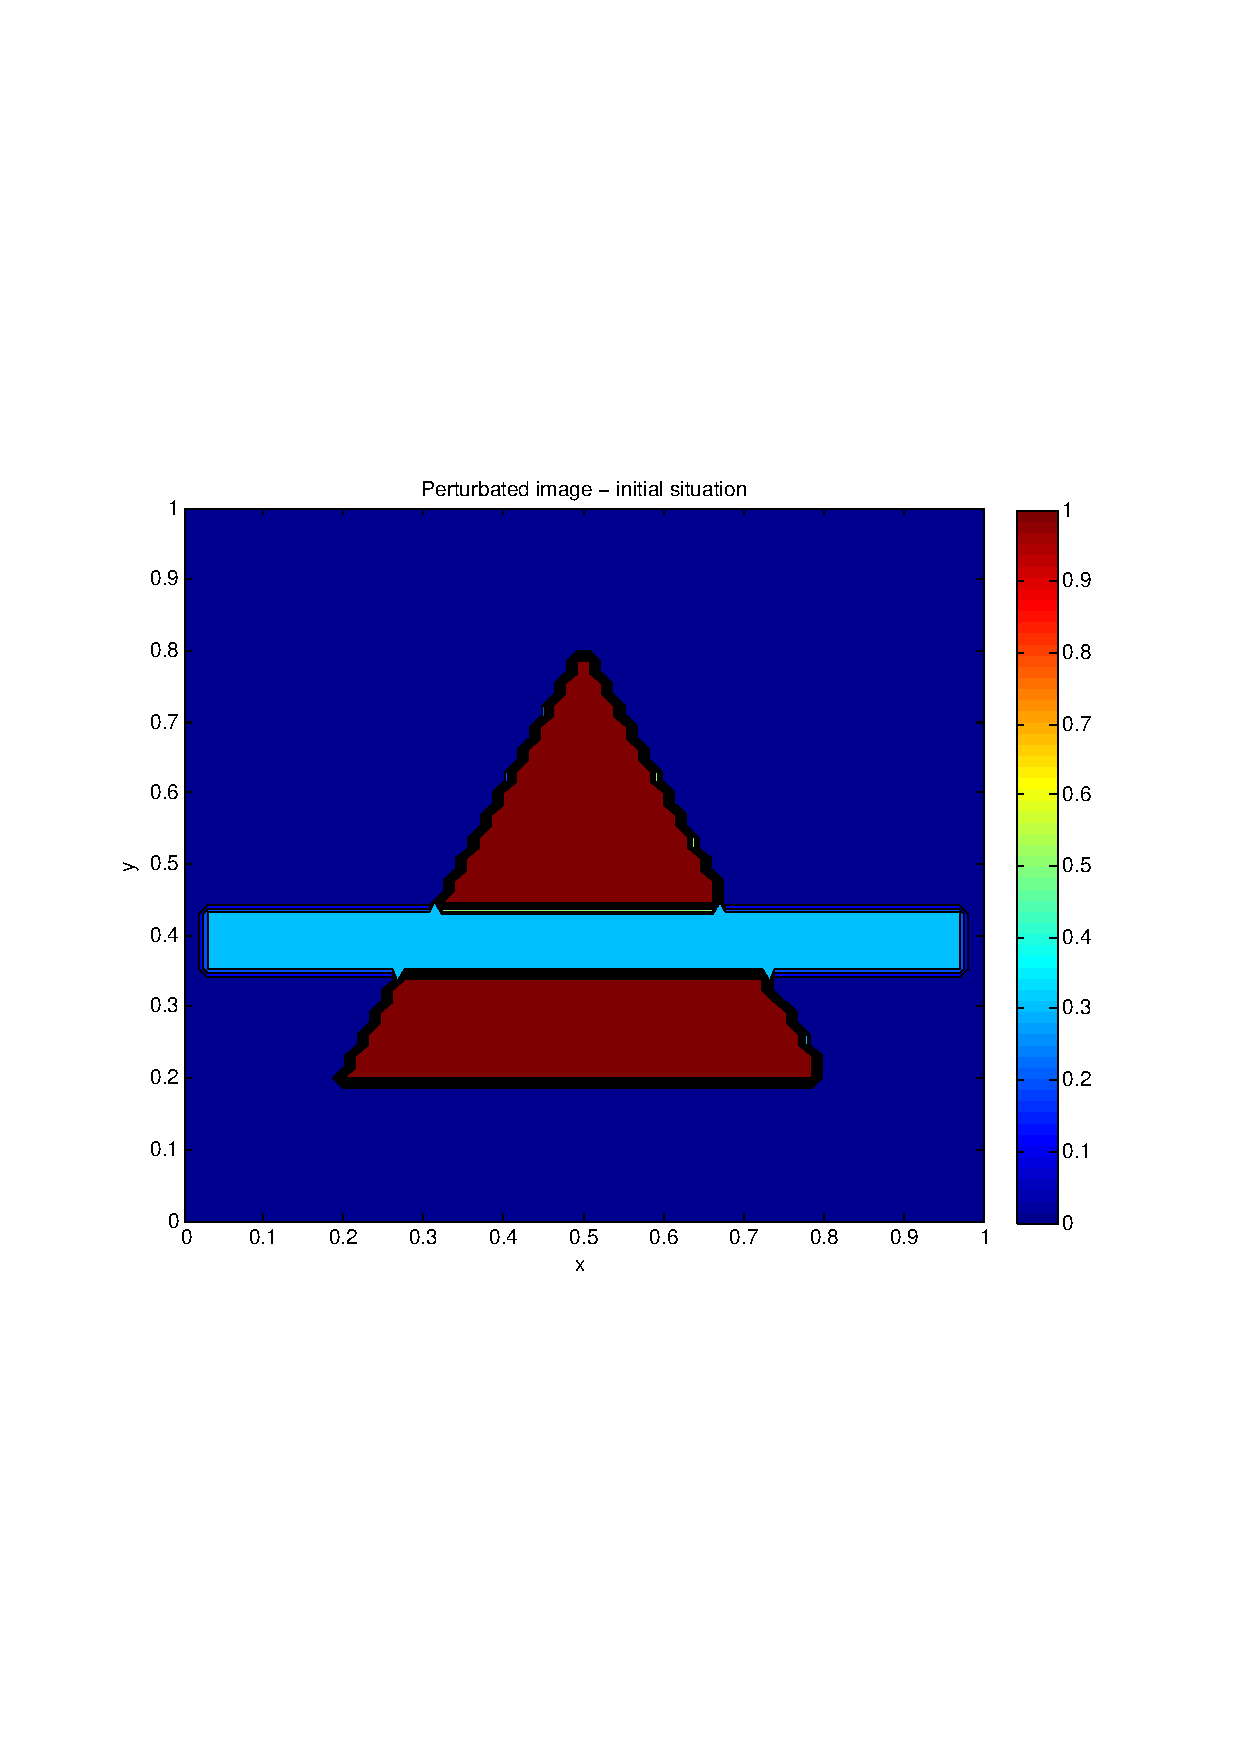
\includegraphics[width=11cm,height=15cm]{NUM_RES/CH_INPAINTING/triangle_N_64_initial.pdf}
\end{center}
\vskip -3.cm
\caption{Inpainting with C-H. $\Delta t=0.001$, $\epsilon=0.05$, $N=64$ - Initial inpainted image}
\label{}
\end{figure}
%%%%%%%%%%%%%%%%%%%%%%%%%%%%%%%%%%%%%
\begin{figure}[!h]
\vskip -1.5cm
\begin{center}
\includegraphics[width=6.2cm,height=6cm]{NUM_RES/CH_INPAINTING/triangle_Tfinal_N_64_DT_0p001.eps}
\includegraphics[width=6.2cm,height=6cm]{NUM_RES/CH_INPAINTING/RSS_triangle_Tfinal_N_64_DT_0p001.eps}
\end{center}
\vskip -.5cm
\caption{Inpainting with C-H. $\Delta t=0.001$, $\epsilon=0.05$, $N=64$ - Restored triangle at $T=0.1$, classical (left) RSS method (right)}
\label{}
\end{figure}
\begin{figure}[!h]
\vskip -1.5cm
\begin{center}
\includegraphics[width=6.2cm,height=6cm]{NUM_RES/CH_INPAINTING/triangle_final_N_64_DT_0p001.eps}
\includegraphics[width=6.2cm,height=6cm]{NUM_RES/CH_INPAINTING/RSS_triangle_final_N_64_DT_0p001.eps}
\end{center}
\vskip -.5cm
\caption{Inpainting with C-H. $\Delta t=0.001$, $\epsilon=0.05$, $N=64$ - Restored triangle with thresholding at $T=0.1$, classical (left) RSS method (right)}
\label{}
\end{figure}

\clearpage
 %%%%%%%%%%%%%%%%%%%%%%%%%%%%%%%%%%%%%%%%%%%%
 %Circle example
 %%%%%%%%%%%%%%%%%%%%%%%%%%%%%%%%%%%%%%%%%%%%
\begin{figure}[!h]
\vskip -0.6cm
\begin{center}
\includegraphics[width=7cm,height=6cm]{NUM_RES/CH_INPAINTING/RSS_cercles_N_128_initial.eps}
\includegraphics[width=7cm,height=6cm]{NUM_RES/CH_INPAINTING/RSS_cercles_t0p005_N_128_DT_0p001.eps}

\end{center}
%\vskip -3.cm
\caption{Inpainting with C-H. $\Delta t=0.001$, $\epsilon=0.05$, $N=128$ - Initial inpainted image, left ($t=0$), right ($t=0.005$)}
\label{}
\end{figure}
%

\begin{figure}[!h]
\vskip -0.6cm
\begin{center}
\includegraphics[width=7cm,height=6cm]{NUM_RES/CH_INPAINTING/RSS_cercles_t0p008_N_128_DT_0p001.eps}
\includegraphics[width=7cm,height=6cm]{NUM_RES/CH_INPAINTING/RSS_cercles_t0p01_N_128_DT_0p001.eps}
\end{center}
%\vskip -3.cm
\caption{Inpainting with C-H. $\Delta t=0.001$, $\epsilon=0.05$, $N=128$ -  image at $t=0.008$ (left)
and at $t=0.01$ (right)}
\label{}
\end{figure}
%
\begin{figure}[!h]
\vskip -0.6cm
\begin{center}
\includegraphics[width=7cm,height=6cm]{NUM_RES/CH_INPAINTING/RSS_cercles_t0p02_N_128_DT_0p001.eps}
\includegraphics[width=7cm,height=6cm]{NUM_RES/CH_INPAINTING/RSS_cercles_Tfinal_N_128_DT_0p001.eps}
\end{center}
%\vskip -3.cm
\caption{Inpainting with C-H. $\Delta t=0.001$, $\epsilon=0.05$, $N=128$ -  image at $t=0.02$ (left)
and at $t=0.1$ (right). RSS cCheme}
\label{}
\end{figure}
\begin{figure}[!h]
\vskip -0.6cm
\begin{center}
\includegraphics[width=7cm,height=6cm]{NUM_RES/CH_INPAINTING/RSS_cercles_final_N_128_DT_0p001.eps}
\end{center}
%\vskip -3.cm
\caption{Inpainting with C-H. $\Delta t=0.001$, $\epsilon=0.05$, $N=128$ -  thresholded image at $t=0.1. RSS Scheme}
\label{}
\end{figure}
\clearpage
\subsubsection{3D Inpainting}
%%%%%%%%%%%%%%%%%%%%%%%%%%%%%%%%%%%%%
\begin{figure}[!h]
\vskip 1cm
\begin{center}
\includegraphics[width=7cm,height=6cm]{NUM_RES/CH_INPAINTING/spriral_initial.eps}
\end{center}
%\vskip -3.cm
\caption{Inpainting 3D with C-H. $\Delta t=1.e-7$, $\lambda=100000$, $\epsilon=0.05$, $N=20$ - }
\label{}
\end{figure}

\begin{figure}[!h]
\vskip -0.6cm
\begin{center}
\includegraphics[width=7cm,height=6cm]{NUM_RES/CH_INPAINTING/spriral_perturbed.eps}
\end{center}
%\vskip -3.cm
\caption{Inpainting 3D with C-H. $\Delta t=1.e-7$, $\lambda=100000$, $\epsilon=0.05$, $N=20$}
\label{}
\end{figure}

\begin{figure}[!h]
\vskip -0.6cm
\begin{center}
\includegraphics[width=7cm,height=6cm]{NUM_RES/CH_INPAINTING/spriral_corrected.eps}
\end{center}
%\vskip -3.cm
\caption{Inpainting 3D with C-H. $\Delta t=1.e-7$, $\lambda=100000$, $\epsilon=0.05$, $N=20$}
\label{}
\end{figure}



%%%%%%%%%%%%%%%%%%%%%%%%%%%%%%%%%%%%%%%%%%%%
%
%\begin{figure}[!h]
%\begin{center}
%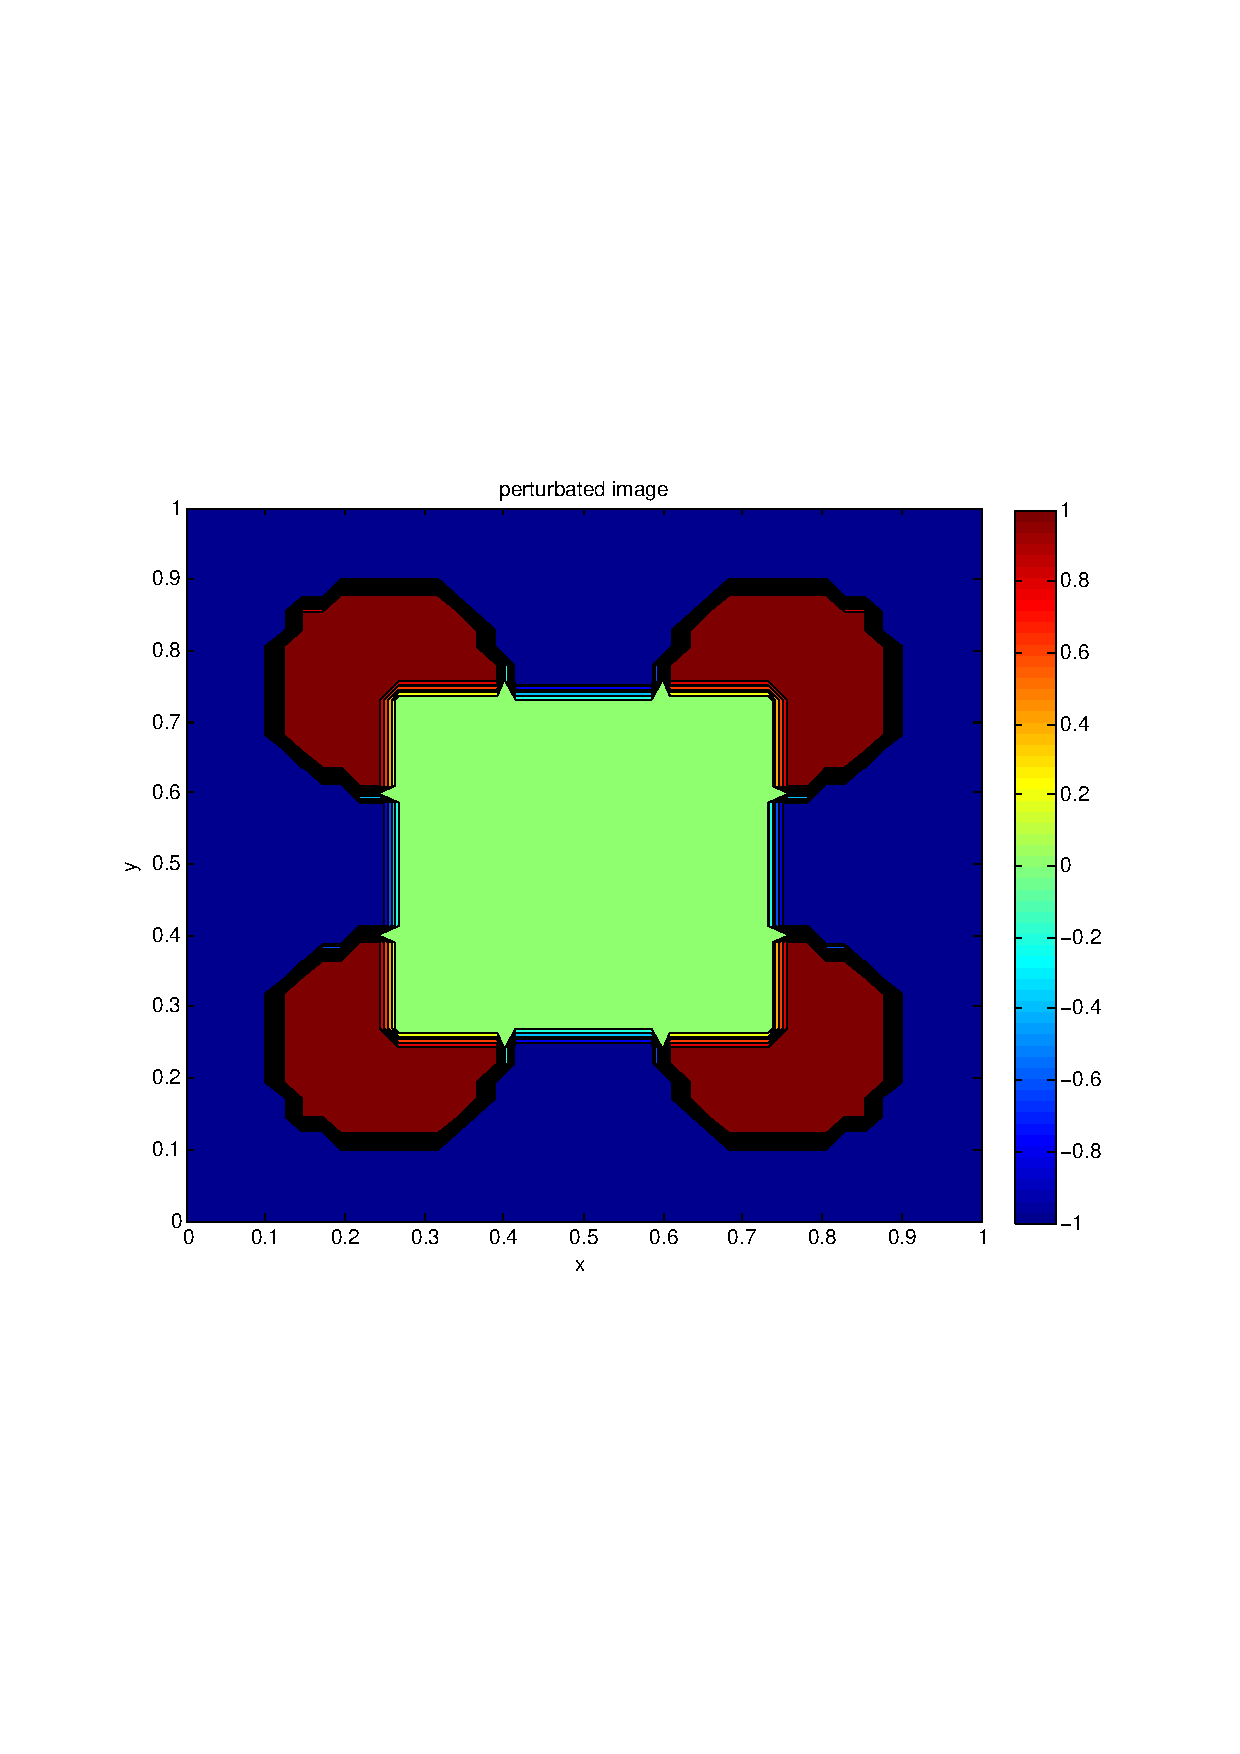
\includegraphics[width=15cm,height=15cm]{NUM_RES/CH_INPAINTING/Inp_CH_RSS_N64_tau2p2_eps0p5_dt0p01.png}
%\vskip -0.5cm
%\caption{Inpainting with C-H. $\Delta t=0.01$, $\epsilon=0.5$, $\tau=2.2$, N=64$ - Initial inpainted image}
%\label{}
%\end{center}
%\end{figure}
%\begin{figure}[!h]
%\begin{center}
%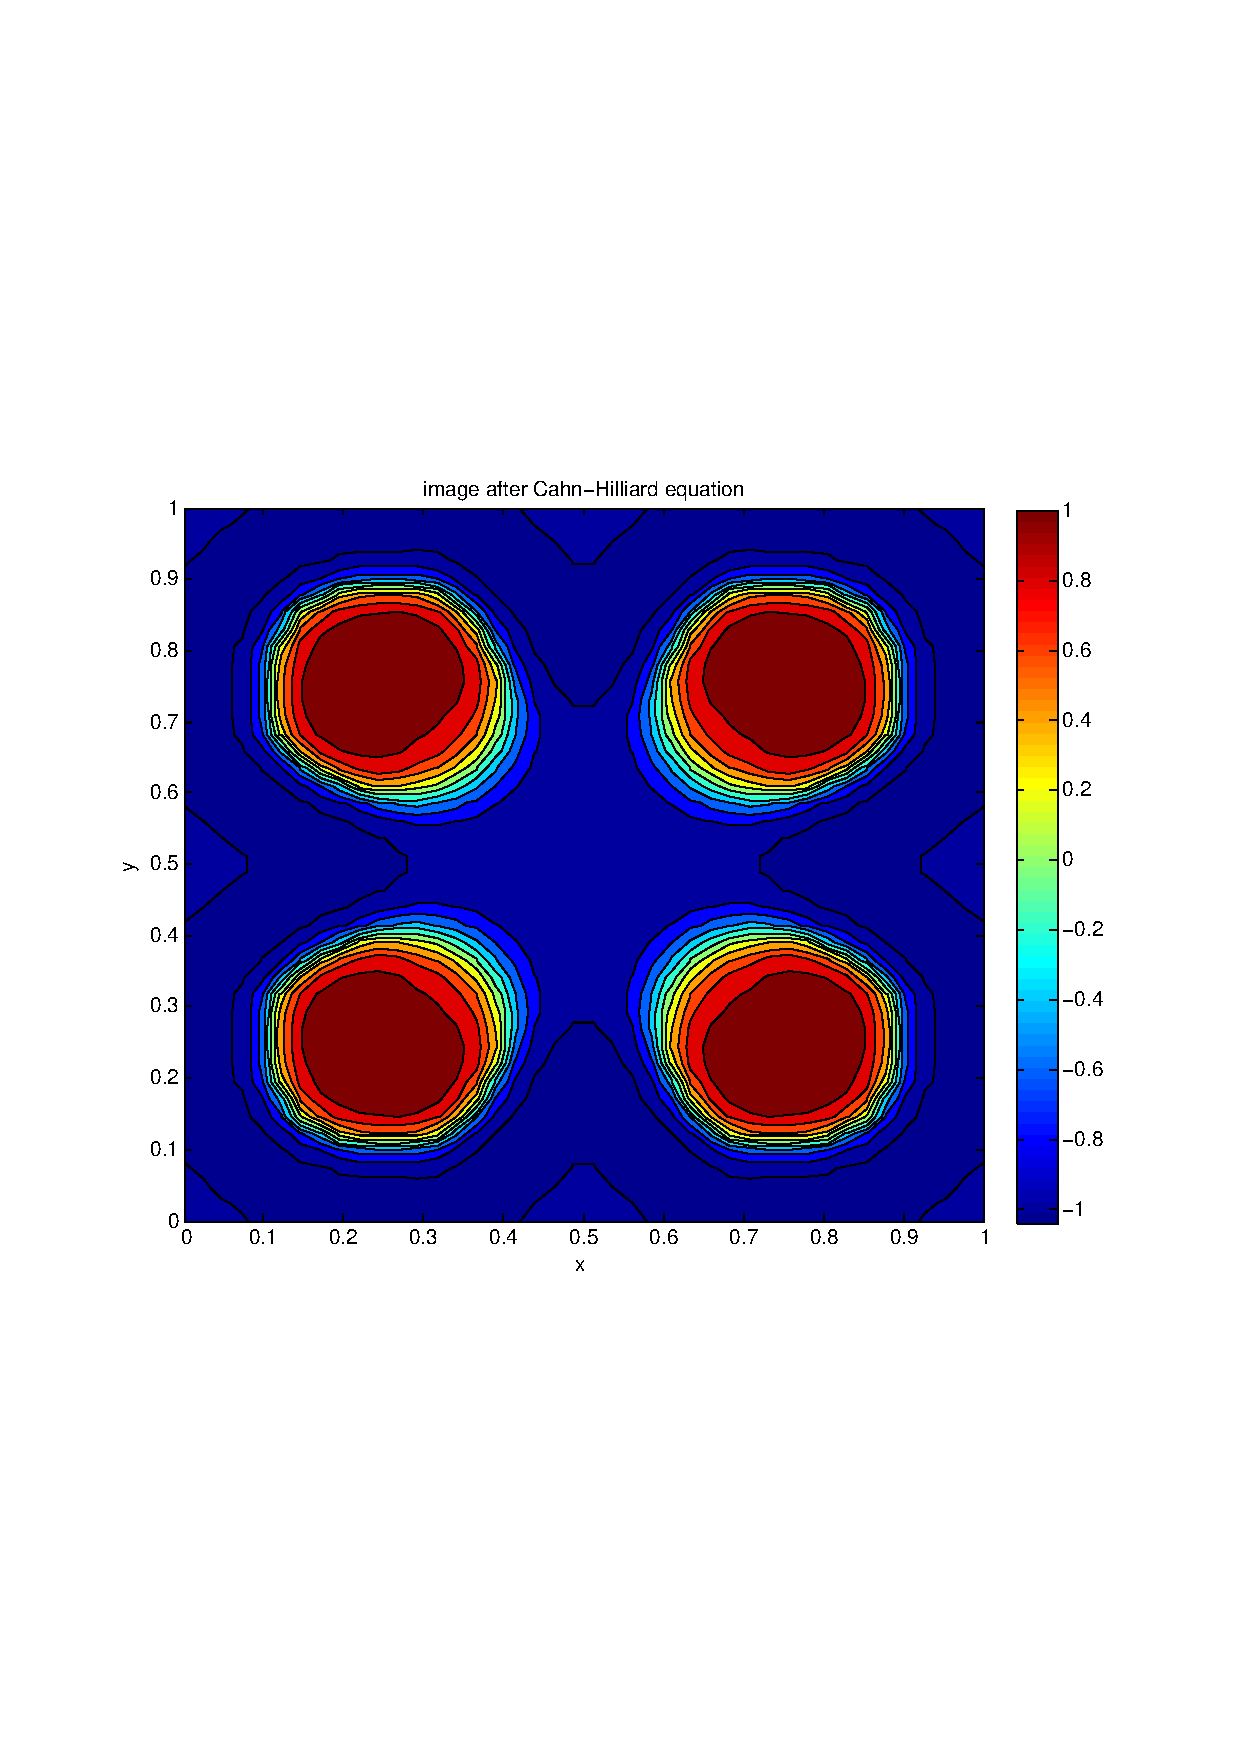
\includegraphics[width=15cm,height=15cm]{NUM_RES/CH_INPAINTING/Inp_final_CH_RSS_N64_tau2p2_eps0p5_dt0p01.png}
%
%\vskip -0.5cm
%\caption{Inpainting with C-H. $\Delta t=0.01$, $\epsilon=0.5$, $\tau=2.2$, N=64$ - final  image cpu=2540.61}
%\label{}
%\end{center}
%\end{figure}
%\begin{figure}[!h]
%\begin{center}
%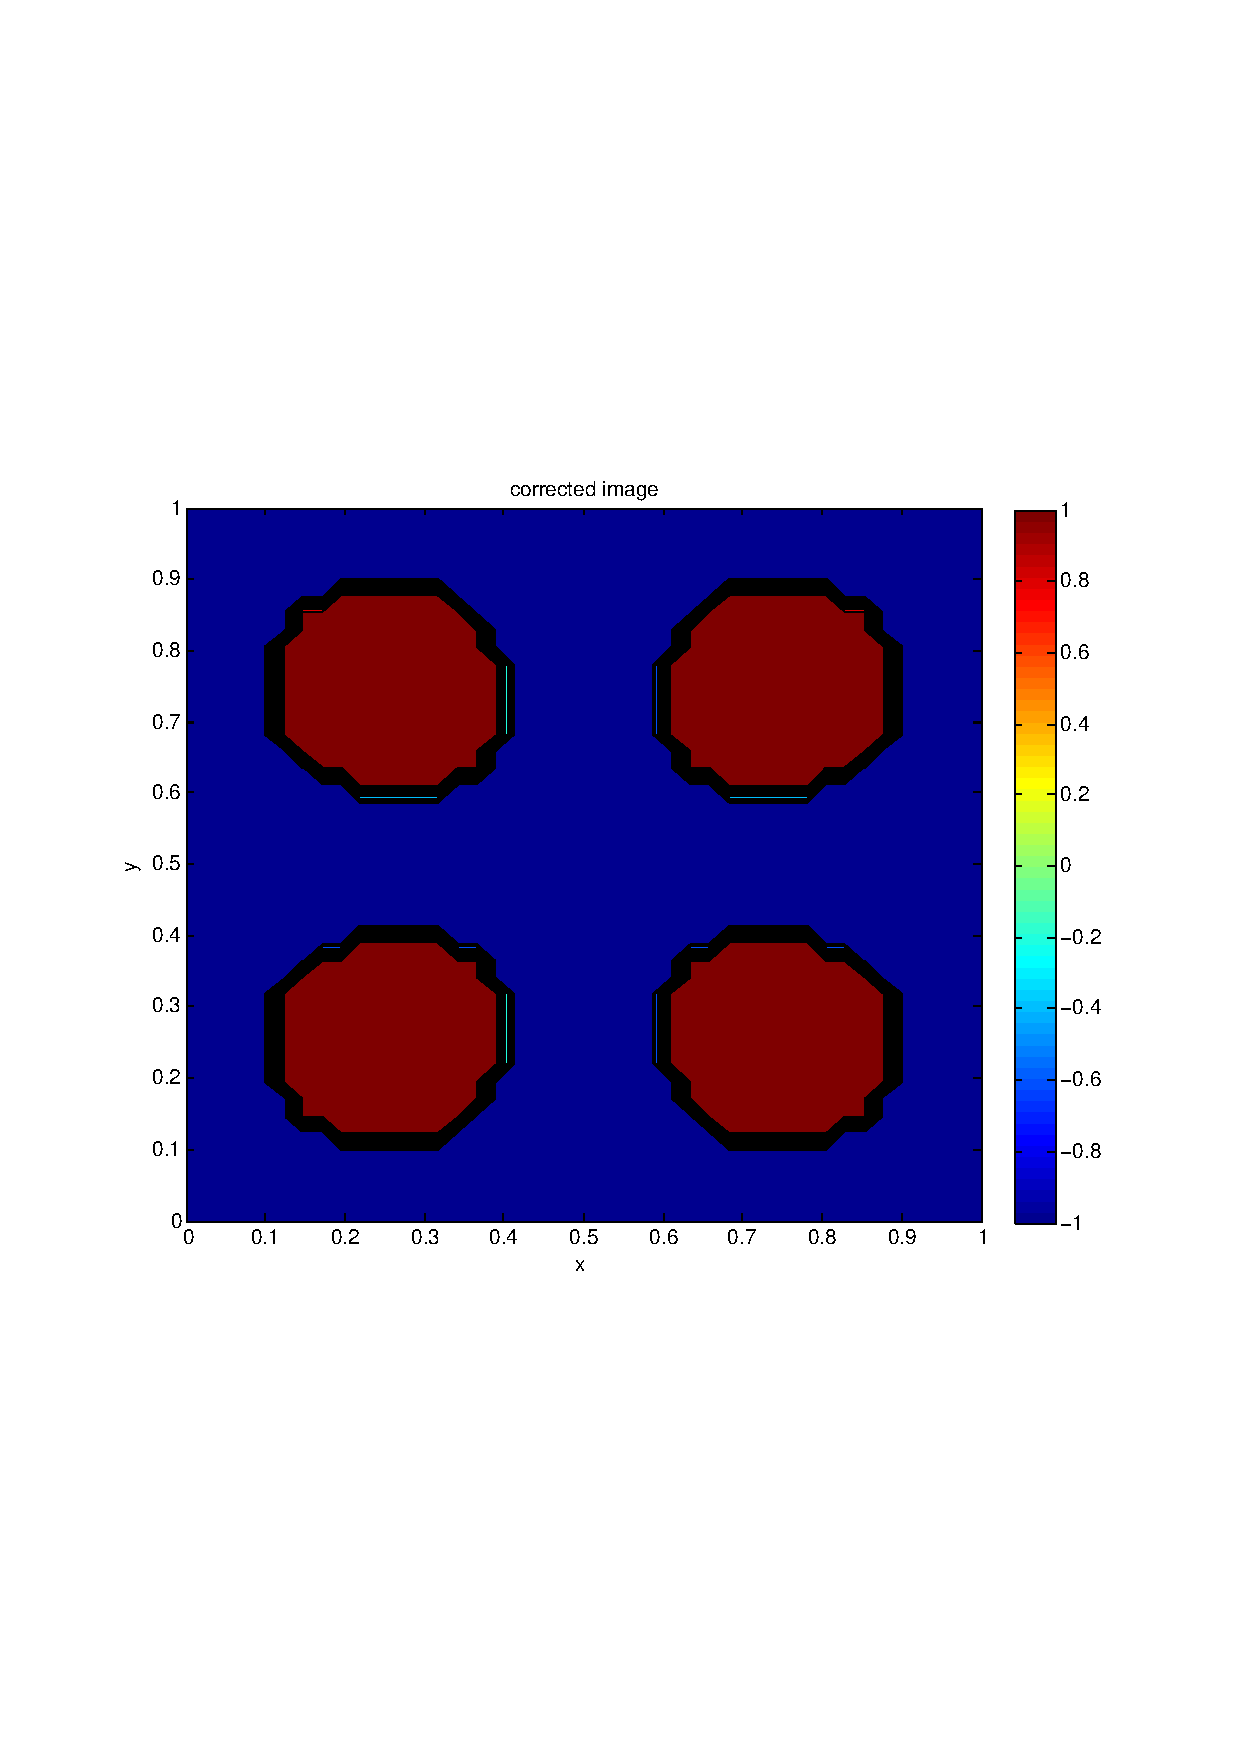
\includegraphics[width=15cm,height=15cm]{NUM_RES/CH_INPAINTING/Inp_final_post_CH_RSS_N64_tau2p2_eps0p5_dt0p01.png}
%\vskip -0.5cm
%\caption{Inpainting with C-H. $\Delta t=0.01$, $\epsilon=0.5$, $\tau=2.2$, N=64$ - final tresholded  image cpu=2540.61}
%\label{}
%\end{center}
%\end{figure}
%%%%%%%%%%%%%%%%%%%%%%%%%%%%%%%%%%%%%%%%%%%%%%%%%
%
%BIBLIOGRAPHY
%
%%%%%%%%%%%%%%%%%%%%%%%%%%%%%%%%%%%%%%%%%%%%%%%%%
\clearpage
\section{Concluding Remarks}
We have introduced stabilized finite differences semi-implicit schemes that allows to simulate fastly high accurate solution of phase fields problems since
the main effort of the computation lies on the efficient solution of sparse linear systems.
\begin{thebibliography}{99}
\bibitem{AllenCahn1} 
S.~M.~Allen, J.~W.~Cahn.
\newblock\emph{Ground State Structures in Ordered Binary Alloys with Second Neighbor
 Interactions}.
\newblock Acta Met. 20, 423 (1972).

\bibitem{AllenCahn2}
S.~M.~Allen, J.~W.~Cahn.
\newblock\emph{A Correction to the Ground State of FCC
Binary Ordered Alloys with First and Second Neighbor Pairwise
Interactions}.
\newblock Scripta Met. 7, 1261 (1973).
\bibitem{AverbuchCohenIsraeli} Amir Averbuch, Albert Cohen et Moshe Israeli : A stable and accurate explicit scheme for
parabolic evolution equations. rapport LAN 1998, unpublished

\bibitem{Bartels} S. Bartels, Numerical Methods for Nonlinear Partial Differential Equations, Springer Series in Computational Mathematics 47, �015

\bibitem{Benes} M. Benes, V. Chalupecky, K. Mikula, 
Geometrical image segmentation by the Allen-Cahn equation,
Applied Numerical Mathematics 51, (2004), 187-205.
\bibitem{Bertozzi1} A. Bertozzi, S. Esedoglu, and A. Gillette, Analysis of a two-scale Cahn--Hilliard model
for binary image inpainting, Multiscale Model. Simul. 6 (2007), 913--936.
\bibitem{Bertozzi2} A. Bertozzi, S. Esedoglu, and A. Gillette, Inpainting of binary images using the Cahn-
Hilliard equation, IEEE Trans. Image Proc. (2007), 285--291.

\bibitem{BrachetChehabJSC} Matthieu Brachet, Jean-Paul Chehab,
Stabilized Times Schemes for High Accurate Finite
Differences Solutions of Nonlinear Parabolic Equations, of Scientific Computing, 69 (3), 946--982, 2016

\bibitem{Bosch} J. Bosch, D. Kay, M. Stoll, and A.J. Wathen, Fast solvers for Cahn--Hilliard inpainting,
SIAM J. Imag. Sci. 7 (2013), 67--97.
\bibitem{ChehabFrancoMammeri} J.-P. Chehab, A.A. Franco and Y. Mammeri, Boundary Control of the number of the interfaces for the one-dimensional Allen-Cahn equation, DiscR. Cont. dyn. Syst. Serie S, Volume 10, Number 1, pp 87--100, 2017

\bibitem{CostaDettoriGottliebTemam} B. Costa. L. Dettori, D. Gottlieb and R. Temam,
Time marching techniques for the nonlinear Galerkin method, SIAM J.
SC. comp., 23, (2001), 1, 46-65.
\bibitem{Collatz} L. Collatz, The Numerical Treatment of Differential Equations, 3rd Edition, Springer-Verlag, 1966. 
\bibitem{Diegel} A. E. Diegel,
Numerical Analysis of Convex Splitting Schemes
for Cahn-Hilliard and Coupled Cahn-Hilliard-
Fluid-Flow Equations, PhD thesis, may 2015, University of Tennessee - Knoxville
\bibitem{Elliott} C.M. Elliott, The Chan-Hilliard Model for the Kinetics of Phase Separation, 
{\it in} Mathematical Models for Phase Change Problems, International Series od Numerical Mathematics, Vol. 88, (1989) Birkh\"auser.
\bibitem{ElliottStuart} C.M. Elliott and A. Stuart The global dynamics of discrete semilinear parabolic equations. SIAM J. Numer. Anal. 30 (1993) 1622--1663.
\bibitem{Emmerich} H. Emmerich, The Diffuse Interface Approach in Materials Science Thermodynamic. Concepts and Applications of Phase-Field Models.
 Lecture Notes in Physics Monographs, Springer, Heidelberg, 2003.
\bibitem{Eyre} D. J. Eyre, Unconditionallly Stable One-step Scheme for Gradient Systems,
June 1998, unpublished, http://www.math.utah.edu/eyre/research/methods/stable.ps.
\bibitem{Fakih} H. Fakih, {\it Etude mathematique et numerique de quelques
generalisations de l'equation de Cahn-Hilliard :
Applications a la retouche d'images et a la biologie}, Doctoral Thesis, University of Poitier, december 2014
\bibitem{JiangShi}
J. Jiang, J. Shi.
\newblock\emph{Bistability Dynamics in Structured Ecological Models}.
{\it Spatial Ecology}, Stephen Cantrell, Chris Cosner, Shigui Ruan
ed., CRC Press, 2009
\bibitem{Lee} D. Lee , J-Y Huh , D. Jeong , J. Shin, A.Yun a J. Kim, 
\newblock\emph{Physical, mathematical, and numerical derivations of the Cahn-Hilliard equation.}
Computational Materials Science 81 (2014) 216--225
\bibitem{Lele} S. Lele, Compact Difference Schemes with Spectral Like resolution, J. Comp. Phys., 103,
(1992), 16--2
\bibitem{LiLee} Y. Li, H. G. Lee, D. Jeong, J. Kim,
An unconditionally stable hybrid numerical method for solving the
Allen-Cahn equation, 
Computers and Mathematics with Applications 60 (2010) 1591--1606
\bibitem{LiJeongChoiLeeKim} 
Y. Li, D. Jeong, J. Choi, S. Lee, J. Kim,
Fast local image inpainting based on the Allen-Cahn model,
Digital SignalProcessing37(2015)65�74
\bibitem{MortonMayers} K.M. Morton and D.F. Mayers,
Numerical Solution of Partial Differential Equations:
An Introduction, Cambridge University Press, second Edition (2005)
\bibitem{MPierreARougirel}  M. Pierre and A. Rougirel, Stationary solutions to phase field crystal equations, Math. Methods Appl. Sci., 34 (2011), no. 3, pp. 278--308
\bibitem{Provatras} Nikolas Provatas and Ken Elder, Phase-Field Methods
in Material Science and Engineering, Wiley-VCH
\bibitem{JShenACCH} J. Shen, X. Yang, Numerical Approximations of Allen-Cahn and Cahn-Hilliard Equations. DCDS, Series A, (28), (2010), pp 1669--1691.
\bibitem{TemamBook} R. Temam, Infnite-dimensional dynamical systems in mechanics and physics, 2nd Ed.,
Springer-Verlag, New York, 1997.
\bibitem{TierraGuillenGonzalez} G. Tierra, F. Guill\'en-Gonz\`alez,
\newblock\emph{Numerical methods for solving the Cahn-Hilliard equation and its
applicability to related Energy-based models.} Ne${\hat c}$as
Center for Mathematical Modeling, Preprint no. 2013-035.
\bibitem{ZaiFengHeb} Shuying Zhai, Xinlong Feng, Yinnian Heb, Numerical simulation of the three dimensional Allen?Cahn equation
by the high-order compact ADI method, Computer Physics Communications 185 (2014) 2449?-2455
\end{thebibliography}
\end{document}